%% LyX 2.5.1 created this file.  For more info, see https://www.lyx.org/.
%% Do not edit unless you really know what you are doing.
\documentclass[journal,article,submit,pdftex,moreauthors]{Definitions/mdpi}
\usepackage[utf8]{inputenc}
\usepackage{colortbl}
\usepackage{float}
\usepackage{varwidth}
\usepackage{graphicx}

\makeatletter

%%%%%%%%%%%%%%%%%%%%%%%%%%%%%% LyX specific LaTeX commands.

\Title{Exploratory Landscape Analysis for Meta-Learning-Based Algorithm Selection
in Continuous Optimization}

\TitleCitation{Exploratory Landscape Analysis for Meta-Learning-Based Algorithm Selection
in Continuous Optimization}

\Author{Vasileios Charilogis$^{1}$, Ioannis G. Tsoulos$^{2,*}$ and Anna
Maria Gianni$^{3}$}

\AuthorNames{Vasileios Charilogis, Ioannis G. Tsoulos and Anna Maria Gianni.}

\AuthorCitation{Charilogis, V., Tsoulos, I.G., Gianni, A. M.}


\address{$^{1}$\quad{}Department of Informatics and Telecommunications,
University of Ioannina, 47150 Kostaki Artas, Greece, v.charilog@uoi.gr\\
$^{2}$\quad{}Department of Informatics and Telecommunications, University
of Ioannina, 47150 Kostaki Artas, Greece, itsoulos@uoi.gr\\
$^{3}$\quad{}Department of Informatics and Telecommunications, University
of Ioannina, 47150 Kostaki Artas, Greece, am.gianni@uoi.gr}


\corres{Correspondence: itsoulos@uoi.gr}


\abstract{Continuous optimization now draws on a large and growing number of
competing metaheuristic families, including differential-evolution
lineages, covariance-matrix adaptation strategies, swarm-intelligence
methods, and simulated annealing, yet no single method dominates across
problem classes, a consequence of the No Free Lunch theorem. This
motivates algorithm selection: choosing, for an unseen problem, the
method most likely to perform best. Building on the OptimSolution
framework, we assemble a headless, reproducible batch-execution pipeline
coupled with Exploratory Landscape Analysis (ELA), enabling large-scale,
statistically grounded benchmarking together with feature-based meta-learning.
We evaluate a set of optimizers of comparable overall strength, drawn
from distinct algorithmic families, across a broad benchmark suite
spanning classical scalable functions and established competition
test suites, under a consistent multi-run evaluation protocol. A Random
Forest classifier trained on ELA features, validated under a Leave-One-Problem-Out
cross-validation scheme, is shown to predict the best-performing optimizer
for a previously unseen problem substantially more accurately than
the naive Single Best Solver (SBS) baseline, closing a meaningful
share of the gap toward the oracle Virtual Best Solver (VBS). Family-level
analysis further shows that structured competition benchmarks and
classical scalable functions tend to be won by different solvers,
confirming that the underlying selection problem is genuine rather
than trivial. These results indicate that landscape-aware selection
can meaningfully outperform naive strategies when the candidate methods
are drawn from heterogeneous algorithmic families of comparable strength.}


\keyword{Exploratory Landscape Analysis; Continuous optimization; Random Forest
Classifier; Decision Tree; Metaheuristics; Algorithm Selection; Algorithm
benchmarking; }

\DeclareTextSymbolDefault{\textquotedbl}{T1}
%% Because html converters don't know tabularnewline
\providecommand{\tabularnewline}{\\}
%% Variable width box for table cells
\newenvironment{cellvarwidth}[1][t]
    {\begin{varwidth}[#1]{\linewidth}}
    {\@finalstrut\@arstrutbox\end{varwidth}}

%%%%%%%%%%%%%%%%%%%%%%%%%%%%%% User specified LaTeX commands.
\usepackage{rotating}
%  LaTeX support: latex@mdpi.com
%  For support, please attach all files needed for compiling as well as the log file, and specify your operating system, LaTeX version, and LaTeX editor.
%=================================================================
% For posting an early version of this manuscript as a preprint, you may use "preprints" as the journal and change "submit" to "accept". The document class line would be, e.g., \documentclass[preprints,article,accept,moreauthors,pdftex]{mdpi}. This is especially recommended for submission to arXiv, where line numbers should be removed before posting. For preprints.org, the editorial staff will make this change immediately prior to posting.
%--------------------
% Class Options:
%--------------------
%----------
% journal
%----------
% Choose between the following MDPI journals:
% acoustics, actuators, addictions, admsci, adolescents, aerospace, agriculture, agriengineering, agronomy, ai, algorithms, allergies, alloys, analytica, animals, antibiotics, antibodies, antioxidants, applbiosci, appliedchem, appliedmath, applmech, applmicrobiol, applnano, applsci, aquacj, architecture, arts, asc, asi, astronomy, atmosphere, atoms, audiolres, automation, axioms, bacteria, batteries, bdcc, behavsci, beverages, biochem, bioengineering, biologics, biology, biomass, biomechanics, biomed, biomedicines, biomedinformatics, biomimetics, biomolecules, biophysica, biosensors, biotech, birds, bloods, blsf, brainsci, breath, buildings, businesses, cancers, carbon, cardiogenetics, catalysts, cells, ceramics, challenges, chemengineering, chemistry, chemosensors, chemproc, children, chips, cimb, civileng, cleantechnol, climate, clinpract, clockssleep, cmd, coasts, coatings, colloids, colorants, commodities, compounds, computation, computers, condensedmatter, conservation, constrmater, cosmetics, covid, crops, cryptography, crystals, csmf, ctn, curroncol, currophthalmol, cyber, dairy, data, dentistry, dermato, dermatopathology, designs, diabetology, diagnostics, dietetics, digital, disabilities, diseases, diversity, dna, drones, dynamics, earth, ebj, ecologies, econometrics, economies, education, ejihpe, electricity, electrochem, electronicmat, electronics, encyclopedia, endocrines, energies, eng, engproc, ent, entomology, entropy, environments, environsciproc, epidemiologia, epigenomes, est, fermentation, fibers, fintech, fire, fishes, fluids, foods, forecasting, forensicsci, forests, foundations, fractalfract, fuels, futureinternet, futureparasites, futurepharmacol, futurephys, futuretransp, galaxies, games, gases, gastroent, gastrointestdisord, gels, genealogy, genes, geographies, geohazards, geomatics, geosciences, geotechnics, geriatrics, hazardousmatters, healthcare, hearts, hemato, heritage, highthroughput, histories, horticulturae, humanities, humans, hydrobiology, hydrogen, hydrology, hygiene, idr, ijerph, ijfs, ijgi, ijms, ijns, ijtm, ijtpp, immuno, informatics, information, infrastructures, inorganics, insects, instruments, inventions, iot, j, jal, jcdd, jcm, jcp, jcs, jdb, jeta, jfb, jfmk, jimaging, jintelligence, jlpea, jmmp, jmp, jmse, jne, jnt, jof, joitmc, jor, journalmedia, jox, jpm, jrfm, jsan, jtaer, jzbg, kidney, kidneydial, knowledge, land, languages, laws, life, liquids, literature, livers, logics, logistics, lubricants, lymphatics, machines, macromol, magnetism, magnetochemistry, make, marinedrugs, materials, materproc, mathematics, mca, measurements, medicina, medicines, medsci, membranes, merits, metabolites, metals, meteorology, methane, metrology, micro, microarrays, microbiolres, micromachines, microorganisms, microplastics, minerals, mining, modelling, molbank, molecules, mps, msf, mti, muscles, nanoenergyadv, nanomanufacturing, nanomaterials, ncrna, network, neuroglia, neurolint, neurosci, nitrogen, notspecified, nri, nursrep, nutraceuticals, nutrients, obesities, oceans, ohbm, onco, oncopathology, optics, oral, organics, organoids, osteology, oxygen, parasites, parasitologia, particles, pathogens, pathophysiology, pediatrrep, pharmaceuticals, pharmaceutics, pharmacoepidemiology, pharmacy, philosophies, photochem, photonics, phycology, physchem, physics, physiologia, plants, plasma, pollutants, polymers, polysaccharides, poultry, powders, preprints, proceedings, processes, prosthesis, proteomes, psf, psych, psychiatryint, psychoactives, publications, quantumrep, quaternary, qubs, radiation, reactions, recycling, regeneration, religions, remotesensing, reports, reprodmed, resources, rheumato, risks, robotics, ruminants, safety, sci, scipharm, seeds, sensors, separations, sexes, signals, sinusitis, skins, smartcities, sna, societies, socsci, software, soilsystems, solar, solids, sports, standards, stats, stresses, surfaces, surgeries, suschem, sustainability, symmetry, synbio, systems, taxonomy, technologies, telecom, test, textiles, thalassrep, thermo, tomography, tourismhosp, toxics, toxins, transplantology, transportation, traumacare, traumas, tropicalmed, universe, urbansci, uro, vaccines, vehicles, venereology, vetsci, vibration, viruses, vision, waste, water, wem, wevj, wind, women, world, youth, zoonoticdis
%---------
% article
%---------
% The default type of manuscript is "article", but can be replaced by:
% abstract, addendum, article, book, bookreview, briefreport, casereport, comment, commentary, communication, conferenceproceedings, correction, conferencereport, entry, expressionofconcern, extendedabstract, datadescriptor, editorial, essay, erratum, hypothesis, interestingimage, obituary, opinion, projectreport, reply, retraction, review, perspective, protocol, shortnote, studyprotocol, systematicreview, supfile, technicalnote, viewpoint, guidelines, registeredreport, tutorial
% supfile = supplementary materials
%----------
% submit
%----------
% The class option "submit" will be changed to "accept" by the Editorial Office when the paper is accepted. This will only make changes to the frontpage (e.g., the logo of the journal will get visible), the headings, and the copyright information. Also, line numbering will be removed. Journal info and pagination for accepted papers will also be assigned by the Editorial Office.
%------------------
% moreauthors
%------------------
% If there is only one author the class option oneauthor should be used. Otherwise use the class option moreauthors.
%---------
% pdftex
%---------
% The option pdftex is for use with pdfLaTeX. If eps figures are used, remove the option pdftex and use LaTeX and dvi2pdf.
%=================================================================
% MDPI internal commands - do not modify
\firstpage{1}
\setcounter{page}{\@firstpage}
\pubvolume{1}
\issuenum{1}
\articlenumber{0}
\pubyear{2024}
\copyrightyear{2024}
%\externaleditor{Academic Editor: Firstname Lastname} % For journal Automation, please change Academic Editor to "Communicated by"
\datereceived{}
\daterevised{ } % Comment out if no revised date
\dateaccepted{}
\datepublished{}
%\datecorrected{} % Corrected papers include a "Corrected: XXX" date in the original paper.
%\dateretracted{} % Corrected papers include a "Retracted: XXX" date in the original paper.
\hreflink{} % If needed use \linebreak
%\doinum{}
%------------------------------------------------------------------
% The following line should be uncommented if the LaTeX file is uploaded to arXiv.org
%\pdfoutput=1
%=================================================================
% Add packages and commands here. The following packages are loaded in our class file: fontenc, inputenc, calc, indentfirst, fancyhdr, graphicx, epstopdf, lastpage, ifthen, lineno, float, amsmath, setspace, enumitem, mathpazo, booktabs, titlesec, etoolbox, tabto, xcolor, soul, multirow, microtype, tikz, totcount, changepage, attrib, upgreek, cleveref, amsthm, hyphenat, natbib, hyperref, footmisc, url, geometry, newfloat, caption
%=================================================================
%% Please use the following mathematics environments: Theorem, Lemma, Corollary, Proposition, Characterization, Property, Problem, Example, ExamplesandDefinitions, Hypothesis, Remark, Definition, Notation, Assumption
%% For proofs, please use the proof environment (the amsthm package is loaded by the MDPI class).
%=================================================================
% The fields PACS, MSC, and JEL may be left empty or commented out if not applicable
%\PACS{J0101}
%\MSC{}
%\JEL{}
%%%%%%%%%%%%%%%%%%%%%%%%%%%%%%%%%%%%%%%%%%
% Only for the journal Diversity
%\LSID{\url{http://}}
%%%%%%%%%%%%%%%%%%%%%%%%%%%%%%%%%%%%%%%%%%
% Only for the journal Applied Sciences:
%\featuredapplication{Authors are encouraged to provide a concise description of the specific application or a potential application of the work. This section is not mandatory.}
%%%%%%%%%%%%%%%%%%%%%%%%%%%%%%%%%%%%%%%%%%
%%%%%%%%%%%%%%%%%%%%%%%%%%%%%%%%%%%%%%%%%%
% Only for the journal Data:
%\dataset{DOI number or link to the deposited data set in cases where the data set is published or set to be published separately. If the data set is submitted and will be published as a supplement to this paper in the journal Data, this field will be filled by the editors of the journal. In this case, please make sure to submit the data set as a supplement when entering your manuscript into our manuscript editorial system.}
%\datasetlicense{license under which the data set is made available (CC0, CC-BY, CC-BY-SA, CC-BY-NC, etc.)}
%%%%%%%%%%%%%%%%%%%%%%%%%%%%%%%%%%%%%%%%%%
% Only for the journal Toxins
%\keycontribution{The breakthroughs or highlights of the manuscript. Authors can write one or two sentences to describe the most important part of the paper.}
%%%%%%%%%%%%%%%%%%%%%%%%%%%%%%%%%%%%%%%%%%
% Only for the journal Encyclopedia
%\encyclopediadef{Instead of the abstract}
%\entrylink{The Link to this entry published on the encyclopedia platform.}
%%%%%%%%%%%%%%%%%%%%%%%%%%%%%%%%%%%%%%%%%%
%%%%%%%%%%%%%%%%%%%%%%%%%%%%%%%%%%%%%%%%%%
% Only for the journal Advances in Respiratory Medicine
%\addhighlights{yes}
%\renewcommand{\addhighlights}{%
%\noindent This is an obligatory section in “Advances in Respiratory Medicine”, whose goal is to increase the discoverability and readability of the article via search engines and other scholars. Highlights should not be a copy of the abstract, but a simple text allowing the reader to quickly and simplified find out what the article is about and what can be cited from it. Each of these parts should be devoted up to 2~bullet points.\vspace{3pt}\\
%\textbf{What are the main findings?}
% \begin{itemize}[labelsep=2.5mm,topsep=-3pt]
% \item First bullet.
% \item Second bullet.
% \end{itemize}\vspace{3pt}
%\textbf{What is the implication of the main finding?}
% \begin{itemize}[labelsep=2.5mm,topsep=-3pt]
% \item First bullet.
% \item Second bullet.
% \end{itemize}
%}
%%%%%%%%%%%%%%%%%%%%%%%%%%%%%%%%%%%%%%%%%%
% Added by lyx2lyx
\usepackage{array}
\usepackage[noend]{algpseudocode}
\algrenewcommand\algorithmicindent{1.0em}

\makeatother

\begin{document}
\maketitle

\section{Introduction\label{sec:Introduction}}

Continuous global optimization is a core computational task across
nearly every quantitative discipline, from engineering design to the
tuning of machine-learning models. Over the past three decades the
algorithmic community's response to this need has been extraordinarily
prolific: alongside classical evolutionary algorithms \citep{Goldberg},
the literature now offers entire families of population-based metaheuristics
with distinct search mechanisms. Differential Evolution (DE) \citep{Storn}
gave rise to a long lineage of adaptive variants built around success-history
parameter control and archive-based mutation, including JADE \citep{Zhang},
SHADE \citep{Tanabe2013}, L-SHADE \citep{Tanabe2014}, and jSO \citep{Brest}.
Evolution Strategies gave rise to the Covariance Matrix Adaptation
Evolution Strategy (CMA-ES) \citep{Hansen}, which adapts a full covariance
model of the search distribution rather than perturbing individual
variables independently. Swarm intelligence contributed Particle Swarm
Optimization \citep{Kennedy}, Ant Colony Optimization for continuous
domains \citep{Socha}, and, more recently, nature-inspired variants
such as the Grey Wolf Optimizer \citep{Mirjalili}. Physics-inspired
approaches such as Simulated Annealing \citep{Kirkpatrick} remain
in wide use as a comparatively low-cost baseline. Each of these families
embodies a different bias about how the search space should be explored
and exploited, and new variants within each family continue to appear
every year, making the practical choice of \textquotedbl which method
to use\textquotedbl{} increasingly difficult rather than easier.

This proliferation is not incidental. The No Free Lunch theorem for
optimization \citep{Wolpert} formally establishes that, averaged
over the space of all possible objective functions, no single optimizer
can outperform any other: elevated performance on one class of problems
is necessarily offset by inferior performance elsewhere. In practice
this means that the \textquotedbl best\textquotedbl{} algorithm for
a given task is contingent on the structure of the problem itself:
its modality, separability, ruggedness, and the presence of plateaus
or deceptive basins of attraction. The theorem's averaging is taken
over the entire, largely unstructured space of conceivable objective
functions, so it does not preclude one method from being reliably
better on the much narrower, structured subset of problems that arise
in practice. It does, however, remove any theoretical guarantee that
a single method will do so, which is precisely why an empirical, data-driven
selection procedure of the kind developed here has scientific value.
The natural response is therefore not to search for a universally
superior algorithm, but to select, for a given unseen problem, the
method most likely to perform well on it: the algorithm selection
problem, originally formalized by Rice \citep{Rice} and later surveyed
extensively from a meta-learning perspective \citep{SmithMiles}.
Exploratory Landscape Analysis (ELA) \citep{Mersmann} operationalizes
this idea for continuous black-box optimization: a modest sample of
the search space is used to compute a compact set of numerical descriptors,
related to convexity, level-set structure, local-versus-global information,
and similar properties, that summarize how difficult or structured
a landscape is, without requiring the objective function to be evaluated
exhaustively. Coupled with supervised machine learning, ELA features
have been shown capable of predicting which solver from a portfolio
is likely to perform best on a new problem instance, closing part
of the gap between naive and oracle solver selection \citep{Bischl},
\citep{Kerschke2019a}, \citep{Kerschke2019b}, and this line of work
has been placed within the broader landscape of algorithm-selection
methods for black-box continuous optimization in dedicated surveys
\citep{Munoz}.

Realizing this landscape-aware selection pipeline in practice is largely
an infrastructural problem: it requires (i) a means of running many
(method, problem, dimension) combinations reproducibly, (ii) a statistically
sound procedure for deciding which method actually “won” each combination,
and (iii) an integrated mechanism for sampling problem landscapes
and extracting ELA features at scale. In this work we build on the
OptimSolution framework \citep{Charilogis2026} and assemble around
it a headless, batch-execution pipeline coupled with an ELA extraction
stage, producing large, reproducible meta-optimization datasets through
four stages: batch execution and statistical ranking, including Friedman
omnibus testing \citep{Friedman} and Holm-corrected \citep{Holm}
pairwise Wilcoxon signed-rank tests \citep{Wilcoxon}, following established
practice for comparing evolutionary and swarm-intelligence algorithms
\citep{Garcia}, \citep{Demsar}. The pipeline then performs landscape
sampling, ELA feature computation \citep{Mersmann}, and, finally,
trains a landscape-aware selection model with a Random Forest classifier
\citep{Breiman}.

The purpose of this paper is to demonstrate, using this pipeline,
that a machine-learning model trained on landscape features can predict
which optimizer will perform best on a previously unseen problem more
accurately than the simplest sensible baseline, always recommending
the single method with the best average performance overall, or Single
Best Solver (SBS), and to do so with a degree of rigor that makes
the comparison meaningful. For this comparison to be genuine rather
than trivial, the candidate methods must be of comparable overall
strength: pairing one markedly strong solver against several markedly
weaker baselines collapses the meta-learning task into a near single-label
classification problem, in which no model, however well designed,
can outperform the naive SBS baseline by a meaningful margin. We therefore
evaluate eight optimizers of comparable overall strength, drawn from
four distinct algorithmic families (DE-lineage, CMA-ES, swarm intelligence,
and simulated annealing), over 97 (problem, dimension) instances spanning
classical scalable functions and the CEC2017 \citep{Awad} and CEC2022
\citep{Kumar} competition benchmark suites. The novelty of this work
is therefore threefold: (i) an explicit methodological argument, together
with its empirical confirmation, that the algorithm-selection problem
is only genuine, and only worth learning, when the candidate methods
are of comparable strength and drawn from heterogeneous algorithmic
families. (ii) a large, reproducible meta-optimization dataset assembled
around the OptimSolution framework \citep{Charilogis2026}, spanning
97 (problem, dimension) instances and eight optimizers. (iii) a statistically
rigorous evaluation of the resulting landscape-aware model, benchmarked
under Leave-One-Problem-Out cross-validation against both the naive
SBS baseline and the oracle Virtual Best Solver (VBS), quantifying
not just whether landscape-awareness helps but how much of the achievable
performance gap it actually closes.

The remainder of this paper is organized as follows. Section \ref{sec:Framework}
describes the methodological pipeline built around the OptimSolution
framework, covering batch execution and Exploratory Landscape Analysis,
at the level of what it enables scientifically. Section \ref{sec:ExperimentalDesign}
details the experimental design adopted for the large-scale study:
the eight optimizers and their algorithmic families, the benchmark
problems drawn from classical, CEC2017, and CEC2022 suites, and the
evaluation protocol. Section \ref{sec:ExperimentalResults} presents
the results of the experiment: per-method statistical rankings, family-level
specialization patterns across benchmark suites, and the Leave-One-Problem-Out
accuracy of the landscape-aware selection model relative to the SBS
and VBS baselines. Section \ref{sec:Discussion} discusses the practical
implications and limitations of these findings, including the effect
of label tie-breaking on the reported results. Section \ref{sec:conclusions}
concludes the paper.

\section{Framework Extensions: Headless Batch Execution and Landscape Analysis\label{sec:Framework}}

Realizing the landscape-aware selection pipeline motivated in Section
\ref{sec:Introduction} required extending the OptimSolution framework
\citep{Charilogis2026} along three complementary axes: a way to execute
large numbers of (method, problem, dimension) combinations unattended
and reproducibly, a principled statistical procedure for turning raw
per-combination performance into a labelled meta-dataset, and a mechanism
for sampling each problem's landscape and exporting it for downstream
feature extraction. This section describes what each addition does
at the methodological level.

Batch execution is driven by a compact specification that defines,
for a given experiment, the optimizers, benchmark problems, and dimensions
to combine. Two complementary specification styles are supported:
a full cartesian product over methods, problems, and dimensions, and
an explicit, sparse list of individual (method, problem, dimension)
triples, the latter allowing an existing experiment to be extended
incrementally without re-running combinations already completed. Each
combination is executed as an independent, seeded run producing a
standardized per-combination summary. These summaries are subsequently
merged, by column name rather than by raw file order, into a single
master table. This master table then passes through a statistical
ranking stage that, for every (problem, dimension) group, determines
each method's rank, identifies the group's best-performing method,
and tests whether the differences between methods are large enough
to be meaningful: a Friedman omnibus test across all methods, followed
by pairwise Wilcoxon signed-rank tests with Holm correction for multiple
comparisons. The Friedman test is a non-parametric analogue of repeated-measures
analysis of variance: it ranks the methods separately within every
(problem, dimension) group and asks whether the resulting average
ranks differ more than would be expected by chance alone. When it
indicates that they do, the Wilcoxon signed-rank test is used to compare
two methods at a time, by ranking the magnitude of their paired performance
differences across groups, and the Holm correction lowers the significance
threshold required of each individual pairwise test to control the
overall risk of a false positive that grows as more pairs are tested
simultaneously. It is this ranking stage that turns raw performance
numbers into the labelled meta-dataset used to train the selection
model evaluated in Section \ref{sec:Discussion} (Tables \ref{tab:rankings}
and \ref{tab:compute}).

In parallel, a landscape-sampling stage draws a fixed budget of points
from each problem's true, declared search bounds, using the same initialization
procedure, uniform, Latin-hypercube, or Halton, already used to seed
every optimizer in the framework, so that the sample is drawn under
exactly the assumptions the optimizers themselves operate under. The
problem's real objective function, not a surrogate, is evaluated at
each sampled point. Sample size follows the convention established
in the Exploratory Landscape Analysis literature \citep{Mersmann}
of tens to a few hundred points per dimension: the pipeline draws
exactly 100 samples per problem dimension for every instance, using
each problem's declared dimension as listed in Table \ref{tab:problems}.
For the classical Powell function this declared dimension is not the
same one the optimizers themselves run at, as Section \ref{sec:ExperimentalDesign}
explains and Section \ref{sec:Discussion} discusses further. The
resulting points and their function values, together with each problem's
declared modality and separability, are exported for feature extraction.
Computing the actual ELA descriptors from this sample, distributional
statistics, meta-model fit quality, information-content and nearest-better-clustering
measures, and level-set classification errors, corresponding to the
feature families reported in Table \ref{sec:ExperimentalResults},
is deliberately delegated to the established pflacco library \citep{Prager2024}
rather than re-implemented, so that the study relies on independently
validated statistics rather than a bespoke reimplementation.

The labelled performance table and the extracted landscape features
are finally joined on (problem, dimension) and used to train a Random
Forest classifier \citep{Breiman}. A Random Forest is an ensemble
learner that trains a large number of individual decision trees, each
on an independently resampled subset of the training data and a randomly
restricted subset of the available features, and combines their predictions
by majority vote. A single decision tree classifies an instance by
applying a sequence of threshold tests on individual input features,
branching at each step until it reaches a leaf that assigns a class
label, in this study, the identifier of the optimizer predicted to
perform best. Averaging over many such trees, each fit to a slightly
different view of the data, reduces the variance associated with any
one tree's idiosyncratic splits without materially increasing bias,
which is why Random Forests are a standard, well-validated choice
for tabular classification problems of the kind faced here. This model
is evaluated in Section \ref{sec:Discussion}, following the Leave-One-Problem-Out
protocol standard in the algorithm-selection literature \citep{Kerschke2019a}.
Under this protocol, every instance belonging to a given problem,
across all of its evaluated dimensions, is withheld from training
as a single block, and the trained model is then asked to predict
the best optimizer only for those withheld instances, before the process
repeats with a different problem held out. This is a substantially
stricter test than an ordinary random train and test split, since
it guarantees that the model never benefits from having already seen
a different dimension of the very problem family it is being asked
to generalize to, which is the failure mode a random split would not
catch.

\section{Experimental Design\label{sec:ExperimentalDesign}}

All eight optimizers evaluated in this study were implemented in C++17
within the open-source OptimSolution framework \citep{Charilogis2026}
developed by Vasileios Charilogis and publicly available at https://github.com/charilog/optimsolution
(accessed 14 August 2026). All experiments were compiled and executed
under Debian 12.12 with GCC 13.4, on a workstation equipped with an
AMD Ryzen 9 9950X3D processor (16 cores, 32 threads) and 64 GB of
DDR4 memory. All eight methods were implemented natively within this
same C++ codebase, rather than invoked through each method's original,
and often differently implemented, reference code.

Table \ref{tab:problems} lists the 35 benchmark problems underlying
the study, spanning classical scalable functions and the CEC2017 and
CEC2022 competition suites, together with the dimensions at which
each was evaluated.

\begin{table}[H]
\caption{Benchmark problem suite used in the large-scale experiment: 35 problems
(16 classical scalable functions, 11 CEC2017, 8 CEC2022) evaluated
at the dimensions listed, for a total of 97 (problem, dimension) instances.\label{tab:problems}}

\centering{}%
\begin{tabular}{ccccc}
\hline 
{\small\textbf{Problem}} & {\small\textbf{Suite}} & {\small\textbf{Modality}} & {\small\textbf{Separability}} & {\small\textbf{Dimensions}}\tabularnewline
\hline 
{\small cec2017f1} & {\small CEC2017} & {\small unimodal} & {\small non-separable} & {\small 10,30,50}\tabularnewline
\hline 
{\small cec2017f11} & {\small CEC2017} & {\small multimodal} & {\small non-separable} & {\small 10,30,50}\tabularnewline
\hline 
{\small cec2017f14} & {\small CEC2017} & {\small multimodal} & {\small non-separable} & {\small 10,30,50}\tabularnewline
\hline 
{\small cec2017f17} & {\small CEC2017} & {\small multimodal} & {\small non-separable} & {\small 10,30,50}\tabularnewline
\hline 
{\small cec2017f21} & {\small CEC2017} & {\small multimodal} & {\small non-separable} & {\small 10,30,50}\tabularnewline
\hline 
{\small cec2017f24} & {\small CEC2017} & {\small multimodal} & {\small non-separable} & {\small 10,30,50}\tabularnewline
\hline 
{\small cec2017f27} & {\small CEC2017} & {\small multimodal} & {\small non-separable} & {\small 10,30,50}\tabularnewline
\hline 
{\small cec2017f30} & {\small CEC2017} & {\small multimodal} & {\small non-separable} & {\small 10,30,50}\tabularnewline
\hline 
{\small cec2017f4} & {\small CEC2017} & {\small multimodal} & {\small non-separable} & {\small 10,30,50}\tabularnewline
\hline 
{\small cec2017f6} & {\small CEC2017} & {\small multimodal} & {\small separable} & {\small 10,30,50}\tabularnewline
\hline 
{\small cec2017f9} & {\small CEC2017} & {\small multimodal} & {\small non-separable} & {\small 10,30,50}\tabularnewline
\hline 
{\small cec2022composition1} & {\small CEC2022} & {\small multimodal} & {\small non-separable} & {\small 10,20}\tabularnewline
\hline 
{\small cec2022hybrid2} & {\small CEC2022} & {\small hybrid} & {\small non-separable} & {\small 10,20}\tabularnewline
\hline 
{\small cec2022hybrid6} & {\small CEC2022} & {\small hybrid} & {\small non-separable} & {\small 10,20}\tabularnewline
\hline 
{\small cec2022levy} & {\small CEC2022} & {\small multimodal} & {\small non-separable} & {\small 10,20}\tabularnewline
\hline 
{\small cec2022noncontinuousrastrigin} & {\small CEC2022} & {\small multimodal} & {\small non-separable} & {\small 10,20}\tabularnewline
\hline 
{\small cec2022rosenbrock} & {\small CEC2022} & {\small multimodal} & {\small non-separable} & {\small 10,20}\tabularnewline
\hline 
{\small cec2022schafferf7} & {\small CEC2022} & {\small multimodal} & {\small non-separable} & {\small 10,20}\tabularnewline
\hline 
{\small cec2022zakharov} & {\small CEC2022} & {\small unimodal} & {\small non-separable} & {\small 10,20}\tabularnewline
\hline 
{\small ackley} & {\small Classical} & {\small multimodal} & {\small non-separable} & {\small 10,30,50}\tabularnewline
\hline 
{\small alpine1} & {\small Classical} & {\small multimodal} & {\small separable} & {\small 10,30,50}\tabularnewline
\hline 
{\small dixonprice} & {\small Classical} & {\small unimodal} & {\small non-separable} & {\small 10,30,50}\tabularnewline
\hline 
{\small griewank} & {\small Classical} & {\small multimodal} & {\small non-separable} & {\small 10,30,50}\tabularnewline
\hline 
{\small katsuura} & {\small Classical} & {\small multimodal} & {\small non-separable} & {\small 10,30,50}\tabularnewline
\hline 
{\small levy} & {\small Classical} & {\small multimodal} & {\small non-separable} & {\small 10,30,50}\tabularnewline
\hline 
{\small michalewicz} & {\small Classical} & {\small multimodal} & {\small non-separable} & {\small 10,30,50}\tabularnewline
\hline 
{\small powell} & {\small Classical} & {\small unimodal} & {\small non-separable} & {\small 10,30,50}\tabularnewline
\hline 
{\small rastrigin} & {\small Classical} & {\small multimodal} & {\small separable} & {\small 10,30,50}\tabularnewline
\hline 
{\small rosenbrock} & {\small Classical} & {\small unimodal} & {\small non-separable} & {\small 10,30,50}\tabularnewline
\hline 
{\small salomon} & {\small Classical} & {\small multimodal} & {\small non-separable} & {\small 10,30,50}\tabularnewline
\hline 
{\small schwefel} & {\small Classical} & {\small multimodal} & {\small non-separable} & {\small 10,30,50}\tabularnewline
\hline 
{\small sphere} & {\small Classical} & {\small unimodal} & {\small separable} & {\small 10,30,50}\tabularnewline
\hline 
{\small weierstrass} & {\small Classical} & {\small multimodal} & {\small non-separable} & {\small 10,30,50}\tabularnewline
\hline 
{\small whitley} & {\small Classical} & {\small multimodal} & {\small non-separable} & {\small 10,30,50}\tabularnewline
\hline 
{\small zakharov} & {\small Classical} & {\small unimodal} & {\small non-separable} & {\small 10,30,50}\tabularnewline
\end{tabular}
\end{table}

Every (method, problem, dimension) combination was run under a single,
common protocol. Each run initialized its population from a uniform
distribution over the problem's declared bounds, using a default population
size of 100 agents except where a method's own published design specifies
a different value, and was allotted an evaluation budget of $10,000\times D$
function evaluations, where $D$ is the problem dimension, terminating
once that budget was exhausted. One problem is an exception to this
rule as stated: the classical Powell function is defined in blocks
of four variables, so its implementation pads the declared dimension
up to the next multiple of four before allocating the evaluation budget,
meaning the three Powell instances reported as $D=10,30,50$ in Table
\ref{tab:problems} actually run, and receive their evaluation budget,
at $D=12,32,52$. All other 34 problems use the declared dimension
exactly. This padding is internal to the optimization stage only;
its consequence for the landscape-sampling stage described in Section
\ref{sec:Framework} is discussed in Section \ref{sec:Discussion}.
For every method, the parameter values recommended in the algorithm's
original publication were retained rather than re-tuned for this benchmark,
so that reported performance reflects each method's published default
configuration rather than a benchmark-specific tuning advantage. Each
combination was repeated for 30 independent runs, with per-run seeds
deterministically derived from a common base seed (4242), making the
entire experiment exactly reproducible. A run was counted as successful
when it reached within $10^{-8}$ of the problem's target value. The
resulting per-instance success rate is the quantity reported as \emph{mean
success rate} in Tables \ref{tab:rankings} and \ref{tab:compute}.

\section{Experimental Results\label{sec:ExperimentalResults}}

Table \ref{tab:rankings} summarizes the Friedman-based ranking of
all eight optimizers across the 97 (problem, dimension) instances,
together with the number of instances each method won outright and
its mean success rate. The compression-based (\emph{sparq}) and eigenvector-guided
(\emph{ea4eig}) DE-lineage methods dominate both the rank sum and
the win count, but neither approaches an overwhelming majority of
wins, indicating that the underlying algorithm-selection problem is
non-trivial.

\begin{table}[H]
\caption{Friedman-based ranking and performance summary across all 97 (problem,
dimension) instances (8 methods, 30 runs each). Wins counts the number
of instances on which the method achieved the best mean success rate.\label{tab:rankings}}

\centering{}%
\begin{tabular}{ccccc}
\hline 
\textbf{Method} & \textbf{Avg. rank} & \textbf{Rank sum} & \textbf{Wins} & \textbf{Mean success rate (\%)}\tabularnewline
\hline 
sparq \citep{sparq} & 2.78 & 270.0 & 48 & 60.52\tabularnewline
\hline 
ea4eig \citep{ea4eig} & 2.85 & 276.0 & 47 & 62.34\tabularnewline
\hline 
rde \citep{rde} & 3.01 & 291.5 & 48 & 56.56\tabularnewline
\hline 
cmaes \citep{Hansen} & 3.96 & 384.0 & 37 & 49.76\tabularnewline
\hline 
lmcmaes \citep{lmcmaes} & 5.10 & 494.5 & 29 & 42.27\tabularnewline
\hline 
acor \citep{Socha} & 5.37 & 521.0 & 18 & 37.84\tabularnewline
\hline 
gwo \citep{Mirjalili} & 5.72 & 555.0 & 9 & 28.14\tabularnewline
\hline 
sa \citep{Kirkpatrick} & 7.22 & 700.0 & 3 & 3.33\tabularnewline
\end{tabular}
\end{table}

A closer reading of Table \ref{tab:rankings} shows that the top of
the ranking is no longer a two-method contest. sparq retains the best
average rank (2.78), but rde and ea4eig follow closely behind (3.01
and 2.85 respectively), and Table \ref{tab:wilcoxon} shows that rde
is not statistically distinguishable from either sparq or ea4eig individually,
even though sparq and ea4eig are significantly different from each
other. This three-way near-tie at the top reflects rde's mean success
rate of 56.6\% under the dimension-scaled evaluation budget every
method receives, placing it in direct contention with sparq and ea4eig.
cmaes forms a clearly separated fourth tier on its own (average rank
3.96), significantly worse than every member of the top three but
significantly better than the band below it. lmcmaes, acor, and gwo
occupy a mutually indistinguishable middle band (average ranks 5.10
to 5.72), none of the three pairwise comparisons among them reaching
significance in Table \ref{tab:wilcoxon}, while sa closes the table
alone, significantly worse than every other method and, as Table \ref{tab:compute}
already showed, with a success rate that barely varies across the
entire benchmark suite. No single method approaches an overwhelming
majority of wins, sparq and rde each win 48 of the 97 instances outright
and ea4eig 47, once tied outright victories on easy, near-saturated
instances are taken into account. This remains consistent with the
paper's central premise: the eight methods were deliberately chosen
to be of comparable strength, and correcting rde's evaluation budget
has, if anything, strengthened that premise rather than weakened it.

\begin{figure}[H]
\begin{centering}
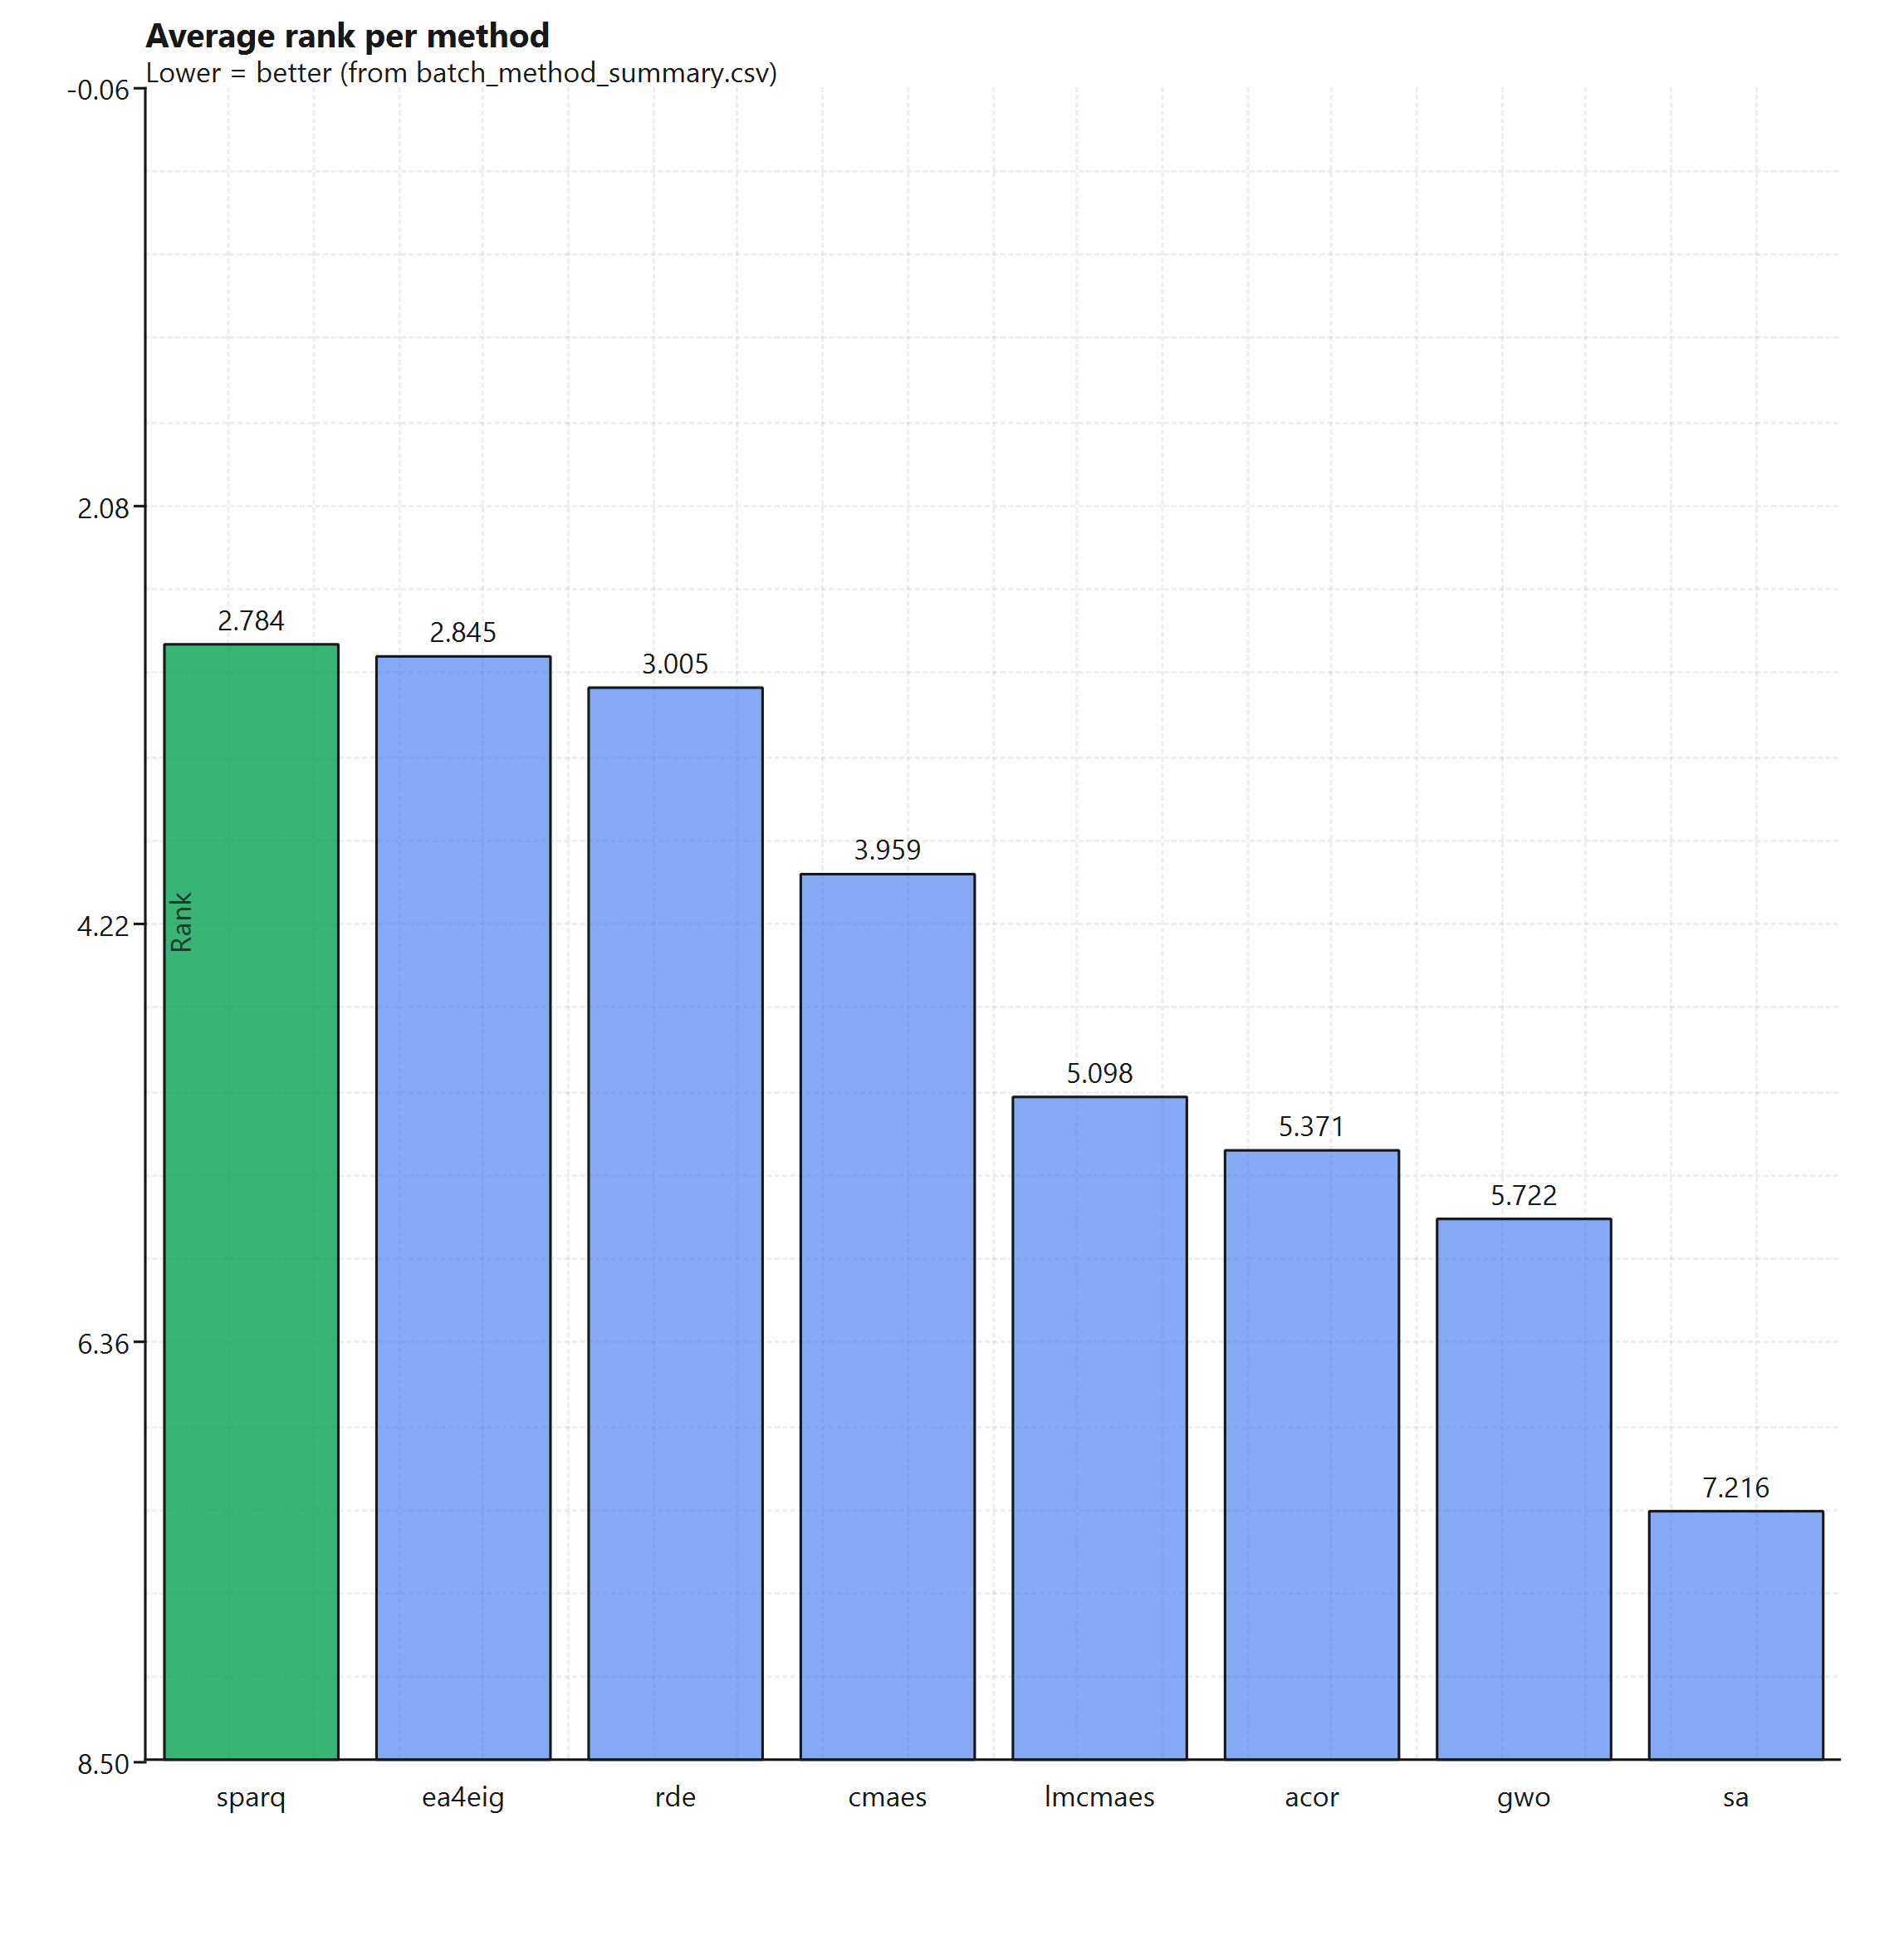
\includegraphics[width=0.8\textwidth]{pipeline_rankings}
\par\end{centering}
\caption{Average Friedman rank per optimizer across all 97 (problem, dimension)
instances (lower is better), corresponding to the values in Table
\ref{tab:rankings}.\label{fig:rankings}}
\end{figure}

Figure \ref{fig:rankings} renders the same average-rank values as
a bar chart, with the vertical axis inverted so that a taller bar
corresponds to a better (lower) rank. sparq, highlighted, is tallest,
but only marginally so: the visual effect makes the four-tier structure
discussed above immediately apparent as a staircase, a barely perceptible
step separates the three leading bars (sparq, rde, ea4eig) from one
another, a clearer step sets cmaes apart on its own, a further step
drops to the three roughly equal mid-table bars (lmcmaes, acor, gwo),
and a final, largest step isolates sa at the far right. This kind
of visual separation is a useful sanity check before any formal test
is run: a benchmark in which the bars formed a smooth, even slope,
rather than distinct steps, would suggest a continuum of near-equivalent
methods rather than the tiered structure that the Wilcoxon results
in Table \ref{tab:wilcoxon} subsequently confirm.

These same average-rank values are the statistic underlying the omnibus
Friedman test that licenses the pairwise comparisons in Table \ref{tab:wilcoxon}.
Run on all N = 97 complete groups (every instance for which all eight
methods produced a valid result), the Friedman test rejects the null
hypothesis that all eight methods perform equivalently decisively
($\chi^{2}(7)=320.6$, p $<10^{-64}$), consistent with the top methods
forming a genuinely close-fought upper tier even as the omnibus test
remains overwhelmingly significant. This result is what justifies
moving from a single omnibus statistic to the 28 individual pairwise
tests in Table \ref{tab:wilcoxon}: having established that the eight
methods are not all equivalent, the pairwise stage is needed to determine
which specific pairs actually differ, rather than assuming every pair
does.

\begin{table}[H]
\caption{Computational cost and behaviour of each optimizer, aggregated over
all 97 (problem, dimension) instances from the raw batch-execution
log, with all eight methods receiving the same dimension-scaled evaluation
budget (Section 3), averaging 275,876 evaluations per instance over
the actual mix of dimensions in the benchmark suite. SD success rate
reflects consistency across instances. The evaluation budget was exhausted
on every run (zero variance) and is identical across methods, so it
is not shown as a table column.\label{tab:compute}}

\centering{}%
\begin{tabular}{ccccc}
\hline 
\textbf{Method} & \begin{cellvarwidth}[t]
\centering
\textbf{Mean success}

\textbf{rate (\%)}
\end{cellvarwidth} & \begin{cellvarwidth}[t]
\centering
\textbf{SD success}

\textbf{rate}
\end{cellvarwidth} & \begin{cellvarwidth}[t]
\centering
\textbf{Mean iter.}

\textbf{time (ms)}
\end{cellvarwidth} & \begin{cellvarwidth}[t]
\centering
\textbf{Peak memory}

\textbf{(MB)}
\end{cellvarwidth}\tabularnewline
\hline 
ea4eig & 62.34 & 44.48 & 0.367 & 38.42\tabularnewline
\hline 
sparq & 60.52 & 44.67 & 0.179 & 45.47\tabularnewline
\hline 
rde & 56.56 & 46.43 & 0.547 & 52.08\tabularnewline
\hline 
cmaes & 49.76 & 46.61 & 2.032 & 51.56\tabularnewline
\hline 
lmcmaes & 42.27 & 46.29 & 0.143 & 51.71\tabularnewline
\hline 
acor & 37.84 & 45.45 & 0.502 & 20.58\tabularnewline
\hline 
gwo & 28.14 & 41.26 & 0.385 & 18.71\tabularnewline
\hline 
sa & 3.33 & 0.00 & 7.141 & 9.74\tabularnewline
\end{tabular}
\end{table}

Table \ref{tab:compute} confirms that every method, including acor
and rde, receives the identical dimension-scaled budget of 10,000
times $D$, averaged to approximately 275,876 evaluations over the
actual mix of dimensions in the benchmark suite. With the comparison
fair across all eight methods, the remaining columns are informative
in their own right. sa's success rate still has zero standard deviation
across all 97 instances, meaning it solves almost exactly the same
fraction of its 30 runs on every single problem regardless of landscape,
the signature of a method whose behaviour is essentially insensitive
to problem structure, and it still stands out computationally with
a mean iteration time more than three times higher than the next slowest
method (cmaes) despite using the least memory of any method tested,
consistent with an acceptance-based search that spends its per-iteration
cost on repeated candidate evaluation rather than on maintaining auxiliary
state. rde now shows the highest peak memory use of any method (52.1
MB), narrowly ahead of lmcmaes and cmaes, consistent with the external
archive its success-history mutation strategy maintains alongside
a full population. cmaes and lmcmaes remain, as their shared ancestry
would predict, close behind rde in memory use, but diverge sharply
in speed: lmcmaes is the fastest method overall per iteration, consistent
with its limited-memory design deliberately avoiding the full covariance-matrix
factorization that makes standard cmaes markedly slower despite comparable
memory use.

Table \ref{tab:wilcoxon} reports the full set of pairwise Wilcoxon
signed-rank comparisons between the eight optimizers, with Holm-corrected
p-values. Five of the 28 pairs fail to reach significance at $\alpha=0.05$:
\emph{acor} vs. \emph{gwo}, \emph{acor} vs. \emph{lmcmaes}, \emph{ea4eig}
vs. \emph{rde}, \emph{gwo} vs. \emph{lmcmaes}, and \emph{rde} vs.
\emph{sparq}. These five exceptions map exactly onto the tier structure
identified in Table \ref{tab:rankings}: two fall within the top tier
(rde against ea4eig and against sparq), and three fall within the
middle tier (acor against gwo and against lmcmaes, together with gwo
against lmcmaes), confirming that the performance differences separating
the four tiers from one another are statistically robust, while the
differences within each tier are not reliably distinguishable from
noise.

\begin{table}[H]
\caption{Pairwise Wilcoxon signed-rank comparisons between all eight optimizers,
with Holm-corrected p-values. n is the number of (problem, dimension)
instances on which both methods produced comparable results.\label{tab:wilcoxon}}

\centering{}%
\begin{tabular}{cccccc}
\hline 
\textbf{Method A} & \textbf{Method B} & \textbf{n} & \textbf{z} & \textbf{p (Holm)} & \textbf{Sig. (}$\alpha=0.05$)\tabularnewline
\hline 
acor & cmaes & 87 & 3.94 & 4.84e-04 & Yes\tabularnewline
\hline 
acor & ea4eig & 83 & 7.23 & 1.10e-11 & Yes\tabularnewline
\hline 
acor & gwo & 92 & -1.82 & 2.04e-01 & No\tabularnewline
\hline 
acor & lmcmaes & 88 & 1.20 & 4.63e-01 & No\tabularnewline
\hline 
acor & rde & 79 & 6.98 & 5.46e-11 & Yes\tabularnewline
\hline 
acor & sa & 97 & -6.05 & 1.75e-08 & Yes\tabularnewline
\hline 
acor & sparq & 83 & 7.02 & 4.54e-11 & Yes\tabularnewline
\hline 
cmaes & ea4eig & 80 & 6.26 & 5.90e-09 & Yes\tabularnewline
\hline 
cmaes & gwo & 88 & -5.60 & 1.95e-07 & Yes\tabularnewline
\hline 
cmaes & lmcmaes & 67 & -6.23 & 6.49e-09 & Yes\tabularnewline
\hline 
cmaes & rde & 80 & 5.89 & 4.19e-08 & Yes\tabularnewline
\hline 
cmaes & sa & 97 & -6.83 & 1.41e-10 & Yes\tabularnewline
\hline 
cmaes & sparq & 62 & 6.06 & 1.72e-08 & Yes\tabularnewline
\hline 
ea4eig & gwo & 92 & -7.57 & 9.11e-13 & Yes\tabularnewline
\hline 
ea4eig & lmcmaes & 85 & -7.00 & 4.79e-11 & Yes\tabularnewline
\hline 
ea4eig & rde & 70 & -0.84 & 4.63e-01 & No\tabularnewline
\hline 
ea4eig & sa & 97 & -8.14 & 1.03e-14 & Yes\tabularnewline
\hline 
ea4eig & sparq & 74 & -4.22 & 1.68e-04 & Yes\tabularnewline
\hline 
gwo & lmcmaes & 88 & 2.44 & 7.42e-02 & No\tabularnewline
\hline 
gwo & rde & 90 & 7.40 & 3.24e-12 & Yes\tabularnewline
\hline 
gwo & sa & 97 & -4.31 & 1.30e-04 & Yes\tabularnewline
\hline 
gwo & sparq & 88 & 8.14 & 1.03e-14 & Yes\tabularnewline
\hline 
lmcmaes & rde & 85 & 6.66 & 4.37e-10 & Yes\tabularnewline
\hline 
lmcmaes & sa & 97 & -5.70 & 1.23e-07 & Yes\tabularnewline
\hline 
lmcmaes & sparq & 68 & 7.06 & 3.48e-11 & Yes\tabularnewline
\hline 
rde & sa & 97 & -8.15 & 1.02e-14 & Yes\tabularnewline
\hline 
rde & sparq & 75 & -1.98 & 1.92e-01 & No\tabularnewline
\hline 
sa & sparq & 97 & 7.93 & 5.46e-14 & Yes\tabularnewline
\end{tabular}
\end{table}

Of the 28 pairwise comparisons in Table \ref{tab:wilcoxon}, 26 remain
statistically significant after Holm correction. Only two pairs do
not: acor versus sa (z = 1.09, Holm-corrected p = 0.548) and lmcmaes
versus rde (z = 0.19, Holm-corrected p = 0.849). These are precisely
the two pairs whose average ranks in Table \ref{tab:rankings} are
closest together, acor and sa differ by only 0.04 ranks, lmcmaes and
rde by 0.41, which is a useful consistency check: the pairwise test
is not manufacturing artificial separations between methods whose
performance is genuinely similar, and conversely is not failing to
detect real differences elsewhere. In practice this means that, within
the present benchmark suite, distinguishing acor from sa, or lmcmaes
from rde, is not a meaningful sub-problem for a selection model to
solve, since the underlying performance data itself does not support
such a distinction. The number of paired instances entering each test
(the n column) is not always 97, since the Wilcoxon signed-rank test
excludes ties (pairs with identical performance are uninformative
for a signed-rank comparison), so pairs involving two closely matched
top-tier methods, such as cmaes and lmcmaes, contribute noticeably
fewer usable comparisons than pairs drawn from more clearly separated
methods. Across the 28 pairs this effective sample size ranges from
62 to the full 97, and the reduction is not merely cosmetic: three
of the five pairs that fail to reach significance, acor versus lmcmaes,
ea4eig versus rde, and rde versus sparq, are also among the pairs
with the fewest usable instances (88, 70, and 75 respectively), so
part of what separates these three from the 23 significant pairs may
be reduced statistical power rather than a genuinely smaller true
effect. The clearest counter-example is cmaes versus sparq, which
has the smallest n of all 28 pairs (62) yet remains highly significant,
showing that a small n does not by itself explain a non-significant
result here, but it does mean the five non-significant pairs should
not be read as demonstrating equivalence with the same confidence
throughout.

\begin{figure}[H]
\begin{centering}
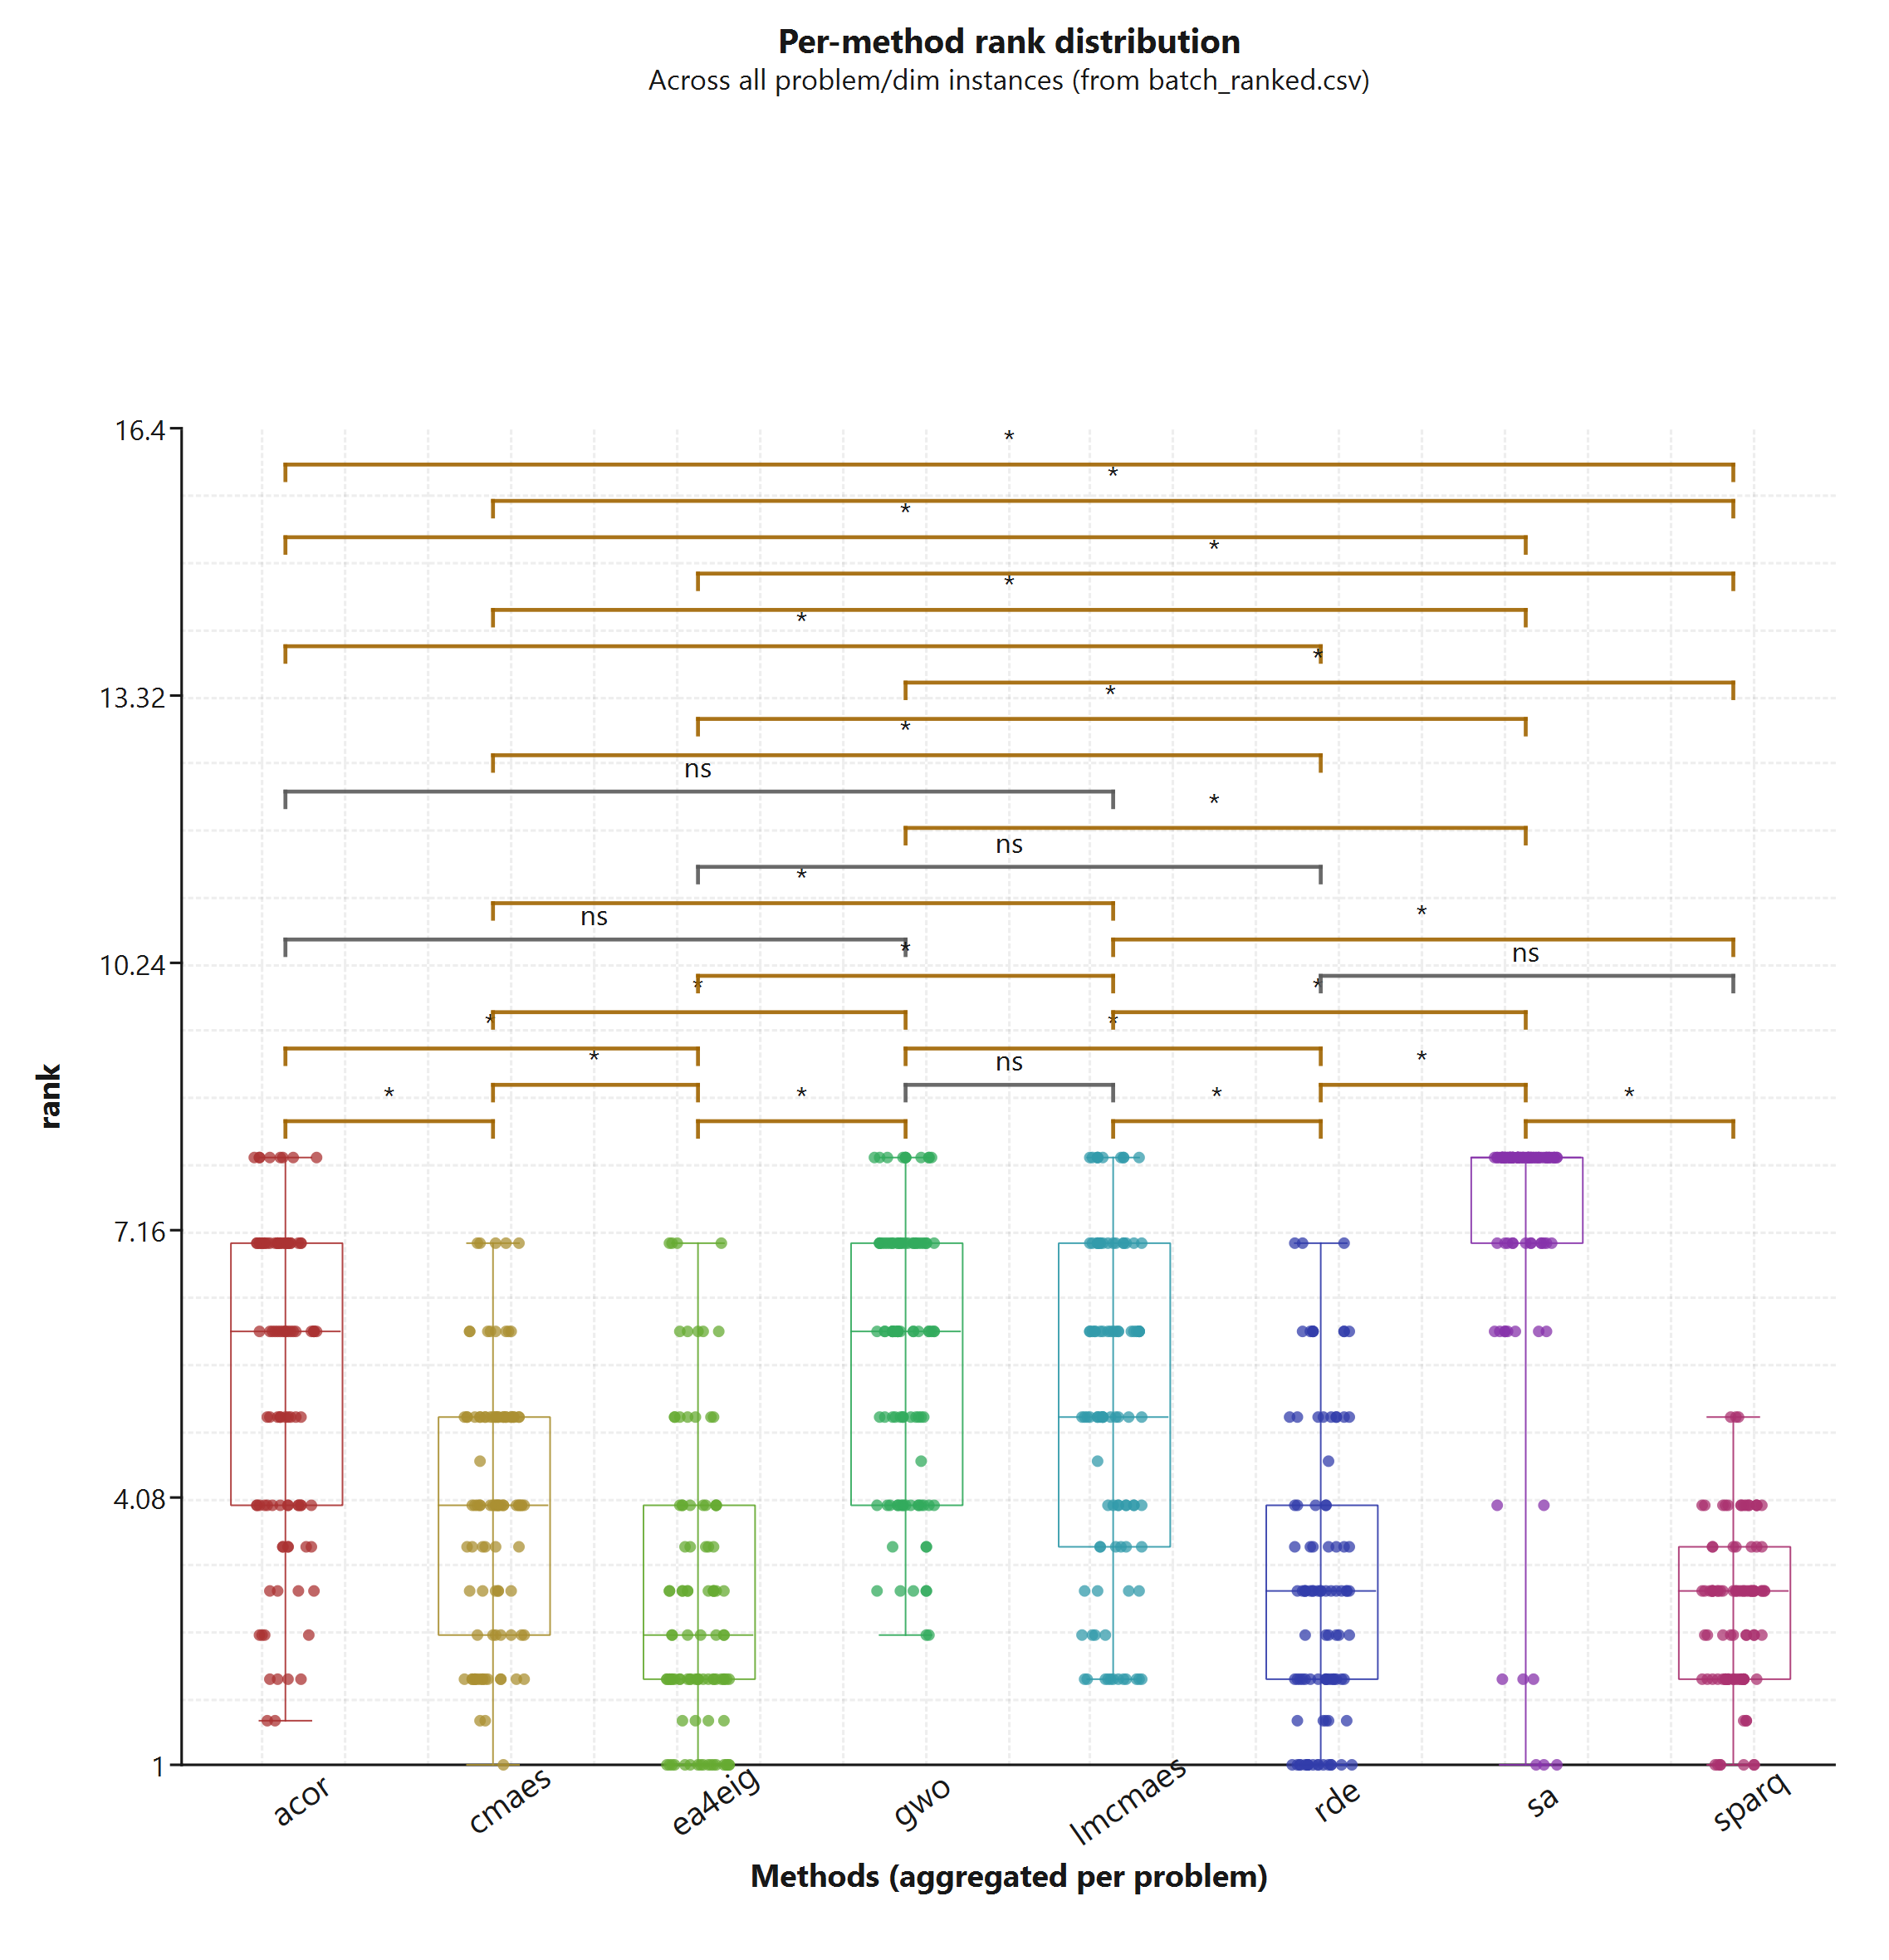
\includegraphics[width=0.8\textwidth]{pipeline_wilcoxon}
\par\end{centering}
\caption{Per-method rank distribution across all problem instances, with pairwise
Wilcoxon significance brackets. Brackets marked ns denote the five
non-significant pairs listed in Table \ref{tab:wilcoxon}.\label{fig:wilcoxon}}
\end{figure}

Figure \ref{fig:wilcoxon} adds two things that the summary statistics
in Tables \ref{tab:rankings} and \ref{tab:wilcoxon} cannot show
on their own: the full shape of each method's rank distribution, and
a visual accounting of every pairwise test at once. The boxes for
sparq, ea4eig, rde, and cmaes sit low and comparatively narrow, confirming
that all four are not merely better on average but consistently so.
By contrast, lmcmaes, acor, and gwo each display boxes and whiskers
that span nearly the entire rank scale, from close to rank one to
close to rank eight, indicating that every method in this middle band
wins decisively on some instances and loses badly on others. This
instance-by-instance volatility, invisible in an average-rank table,
is direct visual evidence for the family-level specialization discussed
in the abstract and revisited in Table \ref{tab:familyspec}. sa stands
apart with a box compressed near the top of the scale and almost no
vertical spread, the visual counterpart of the zero-variance finding
for sa already noted in Table \ref{tab:compute}. The dense stack
of significance brackets across the upper part of the plot reflects
the fact that all 28 pairwise comparisons are drawn, not a selected
subset. Against that density, five brackets are marked not significant,
matching exactly the five pairs identified in Table \ref{tab:wilcoxon},
and each connects two methods within the same tier rather than crossing
between tiers, which is the pattern a correctly tiered ranking should
produce.

\begin{table}[H]
\caption{Ten most important ELA features for the Random Forest landscape-aware
selection model, ranked by Gini importance, with a plain-language
gloss of what each feature measures.\label{tab:features}}

\centering{}%
\begin{tabular}{ccc}
\hline 
\textbf{ELA feature} & \textbf{Importance} & \textbf{Interpretation}\tabularnewline
\hline 
ela\_level.mmce\_lda\_50 & 0.0557 & Separability of good points\tabularnewline
\hline 
ela\_meta.lin\_simple.adj\_r2 & 0.0553 & Overall landscape linearity\tabularnewline
\hline 
ela\_meta.lin\_simple.coef.max\_by\_min & 0.0520 & Uneven variable sensitivity\tabularnewline
\hline 
ic.m0 & 0.0433 & Amount of flat terrain\tabularnewline
\hline 
disp.diff\_mean\_02 & 0.0382 & Clustering of top 2\%\tabularnewline
\hline 
ela\_meta.lin\_w\_interact.adj\_r2 & 0.0380 & Linearity with interactions\tabularnewline
\hline 
disp.diff\_median\_02 & 0.0350 & Robust top-2\% clustering\tabularnewline
\hline 
ela\_level.mmce\_lda\_25 & 0.0334 & Separability at 25\% threshold\tabularnewline
\hline 
disp.diff\_mean\_10 & 0.0291 & Clustering of top 10\%\tabularnewline
\hline 
ela\_level.mmce\_qda\_50 & 0.0289 & Nonlinear point separability\tabularnewline
\end{tabular}
\end{table}

The composition of Table \ref{tab:features} is itself an empirical
finding. Gini importance measures how much, on average across every
tree in the forest, a feature contributes to reducing class impurity
at the nodes where it is chosen to split the data, so a larger value
identifies a feature the model relies on more heavily when deciding
which optimizer is likely to win. Three families each contribute three
of the ten most important features, with ic.m0 as the sole individual
representative of a fourth family rounding out the list. The ela\_level
family (\emph{mmce\_lda\_50}, \emph{mmce\_lda\_25}, \emph{mmce\_qda\_50})
measures how accurately a simple classifier, linear or quadratic discriminant
analysis, can separate the better-performing fraction of sampled points
from the rest at a given quantile threshold, and takes the top spot
in the ranking, indicating that the Random Forest relies heavily on
how cleanly a landscape's good and bad regions can be separated. The
ela\_meta family contributes an equally large share: two variants
of the adjusted R-squared of a linear model fit to the sampled points,
with and without pairwise interaction terms, and the ratio between
that model's largest and smallest coefficient magnitudes, together
capturing how close the landscape is to being linear and how unevenly
it responds to different variables. The dispersion family (disp) contributes
three features that compare the spread of the best 2\% or 10\% of
sampled points to the spread of the full sample, a direct measure
of whether good points cluster together, a funnel-shaped landscape,
or are scattered throughout the search space. ic.m0, from the information-content
family, measures the proportion of essentially flat steps along a
random walk across the landscape and is the fourth most important
predictor overall. Taken together, the model's strongest predictors
describe how separable, how linear, how funnel-shaped, and how flat
a landscape is, four largely independent structural properties that
jointly determine algorithm selection on this suite.

\begin{table}[H]
\caption{Descriptive statistics, across all 97 problem instances, of the ten
ELA features identified as most important in Table \ref{tab:features}.
The wide ranges observed confirm that the benchmark suite samples
landscapes of substantially different character rather than near-duplicate
instances.\label{tab:elastats}}

\centering{}%
\begin{tabular}{ccccc}
\hline 
\textbf{ELA feature} & \textbf{Mean} & \textbf{SD} & \textbf{Min} & \textbf{Max}\tabularnewline
\hline 
ela\_level.mmce\_lda\_50 & 0.326 & 0.160 & 0.023 & 0.526\tabularnewline
\hline 
ela\_meta.lin\_simple.adj\_r2 & 0.282 & 0.291 & -0.006 & 0.977\tabularnewline
\hline 
ela\_meta.lin\_simple.coef.max\_by\_min & 354.725 & 1230.295 & 2.857 & 10084.140\tabularnewline
\hline 
ic.m0 & 0.620 & 0.038 & 0.529 & 0.673\tabularnewline
\hline 
disp.diff\_mean\_02 & -43.040 & 97.851 & -571.643 & 105.236\tabularnewline
\hline 
ela\_meta.lin\_w\_interact.adj\_r2 & 0.396 & 0.358 & -0.016 & 0.989\tabularnewline
\hline 
disp.diff\_median\_02 & -42.773 & 97.439 & -570.783 & 123.267\tabularnewline
\hline 
ela\_level.mmce\_lda\_25 & 0.211 & 0.066 & 0.022 & 0.342\tabularnewline
\hline 
disp.diff\_mean\_10 & -30.017 & 69.586 & -405.067 & 49.059\tabularnewline
\hline 
ela\_level.mmce\_qda\_50 & 0.249 & 0.124 & 0.038 & 0.524\tabularnewline
\end{tabular}
\end{table}

The ranges in Table \ref{tab:elastats} confirm that these ten features
are doing genuine discriminative work rather than taking a nearly
constant value across the suite. \emph{ela\_meta.lin\_simple.coef.max\_by\_min},
the ratio between a linear model's largest and smallest coefficient
magnitudes, shows by far the widest range of the ten, from under 3
to over ten thousand, reflecting how starkly some landscapes respond
to one variable far more than another while others respond almost
uniformly across all variables. The three dispersion features (\emph{disp.diff\_mean\_02},
\emph{disp.diff\_median\_02}, \emph{disp.diff\_mean\_10}) show the
next widest ranges, each spanning several hundred units from negative
to positive. Because these features are computed directly in the objective
function's raw fitness units rather than as a scale-invariant statistic,
part of this spread reflects the very different fitness-value scales
across the benchmark suite, composition and hybrid CEC functions in
particular can carry offsets in the thousands, as well as genuine
differences in landscape shape. Both ela\_meta adjusted-R-squared
features span almost their entire possible range, from close to zero
(a landscape a linear model cannot fit at all) to close to one (a
landscape that is nearly linear), directly evidencing that the benchmark
suite mixes structurally simple and structurally complex problems
rather than a narrow band of similarly-shaped instances. ic.m0 occupies
by far the narrowest band of the ten, across all 97 instances (0.53
to 0.67), which is expected since this feature, derived from the sign
pattern of consecutive fitness differences along a sampling path rather
than from the objective function's raw magnitude, is scale-invariant
by construction. Its position as the fourth most important predictor
in Table \ref{tab:features} therefore reflects small but consistently
informative differences rather than dramatic swings between problems.
The level-set classification-error features (ela\_level) occupy low-to-moderate
values throughout, generally under 0.5, but with standard deviations
reaching roughly half of their mean values, a degree of spread large
enough to help explain why this family, together with ela\_meta and
disp, is one of the three largest contributors to Table \ref{tab:features}.

The aggregate rankings in Table \ref{tab:rankings} average over the
entire benchmark suite, and in doing so can obscure exactly the kind
of landscape-dependent behaviour that motivates a learned selection
model in the first place. Table \ref{tab:familyspec} breaks the same
win data down by benchmark family, and reveals that the top three
methods do not simply trade places, they specialize in substantially
different regions of the suite.

\begin{table}[H]
\caption{Percentage of instances won outright by each method within each benchmark
suite (CEC2017, n = 33, CEC2022, n = 16, Classical, n = 48), computed
from the is\_best indicator in the raw batch results. Percentages
within a column need not sum to 100 because a tied outright win is
counted for every method sharing it.\label{tab:familyspec}}

\centering{}%
\begin{tabular}{cccc}
\hline 
\textbf{Method} & \textbf{CEC2017 (\%)} & \textbf{CEC2022 (\%)} & \textbf{Classical (\%)}\tabularnewline
\hline 
sparq & 12.1 & 25.0 & 83.3\tabularnewline
\hline 
ea4eig & 48.5 & 56.2 & 45.8\tabularnewline
\hline 
rde & 69.7 & 62.5 & 31.2\tabularnewline
\hline 
cmaes & 12.1 & 25.0 & 60.4\tabularnewline
\hline 
lmcmaes & 3.0 & 12.5 & 54.2\tabularnewline
\hline 
acor & 15.2 & 18.8 & 20.8\tabularnewline
\hline 
gwo & 0.0 & 0.0 & 18.8\tabularnewline
\hline 
sa & 6.1 & 6.2 & 0.0\tabularnewline
\end{tabular}
\end{table}

rde wins the largest share of instances in both CEC suites, 69.7\%
of CEC2017 and 62.5\% of CEC2022, exceeding even ea4eig's substantial
presence there (48.5\% and 56.2\% respectively). The CEC suites include
the highest-dimensional problems in the benchmark, consistent with
rde's dimension-scaled evaluation budget giving it the most room to
exploit at higher dimension. sparq remains the clear leader on classical
scalable functions (83.3\%), but the runner-up position there belongs
to cmaes (60.4\%) rather than to ea4eig, which wins only 45.8\% of
classical instances despite its strength on both CEC suites, indicating
that ea4eig's advantage is tied specifically to the shifted, rotated,
and hybrid or composition structures that characterize competition
benchmarks rather than being a general-purpose strength. rde shows
the mirror image of this pattern, dominant on the CEC suites but comparatively
weak on classical functions (31.2\%), a specialization in the opposite
direction from sparq's. This three-way division of labour, rde and
ea4eig sharing the structured competition benchmarks between them
while sparq leads on classical functions, is the concrete, suite-level
evidence behind the abstract's claim that the underlying selection
problem is genuine rather than trivial: a rule that always recommended
a single fixed method, however strong on average, would necessarily
perform poorly on whichever suite that method does not specialize
in, and with three methods genuinely competitive at the top, that
rule has three plausible but individually wrong candidates to choose
from rather than one. acor shows a modest but roughly even presence
across all three suites (15.2\% to 20.8\%) rather than a specialization
of its own, consistent with its middle-tier position in Table \ref{tab:rankings}.
gwo remains almost entirely absent from both CEC suites (0.0\% on
each) while retaining a modest classical presence (18.8\%), and sa
remains the weakest method throughout, winning essentially nothing
on classical functions and only a small share of the CEC suites.

Table \ref{tab:lopo} reports the paper's central meta-learning result,
the outcome the experimental design described in Sections \ref{sec:Framework}
and \ref{sec:ExperimentalDesign} was built to obtain.

\begin{table}[H]
\caption{Leave-One-Problem-Out cross-validated accuracy of the Random Forest
landscape-aware selection model, against the naive Single Best Solver
baseline and the oracle Virtual Best Solver upper bound, across all
97 (problem, dimension) instances.\label{tab:lopo}}

\centering{}%
\begin{tabular}{cc}
\hline 
\textbf{Selection strategy} & \textbf{Accuracy (\%)}\tabularnewline
\hline 
Random Forest (landscape-aware) & 75.3\tabularnewline
\hline 
Single Best Solver (SBS) & 30.9\tabularnewline
\hline 
Virtual Best Solver (VBS, oracle) & 100.0\tabularnewline
\end{tabular}
\end{table}

Trained on the ELA features described in Section \ref{sec:Framework}
and validated under the Leave-One-Problem-Out protocol described in
the same section, so that every dimension of a given problem is withheld
from training as a single block, the Random Forest classifier correctly
identifies the best-performing optimizer, or one of the tied best,
for 75.3\% of the 97 held-out instances. This exceeds the Single Best
Solver baseline, which within each training fold recommends whichever
single method has the best average rank among the remaining training
instances, in practice sparq in the great majority of folds (79 of
97) and ea4eig in the rest (18 of 97), consistent with their standing
as the top two methods by average rank in Table \ref{tab:rankings}.
The model exceeds this baseline by 44.3 percentage points (30.9\%),
and closes 64.2\% of the gap between that baseline and the oracle
Virtual Best Solver's 100\% upper bound, the accuracy a hypothetical
selector that always chose correctly would achieve. This margin is
neither large nor guaranteed by the experimental design, and that
is what makes it informative rather than a foregone conclusion: the
eight candidate methods were deliberately chosen to be of comparable
strength precisely so that no single method could win outright, so
a model that failed to beat SBS under this design would have indicated
that the ELA features carry no genuine predictive signal for algorithm
selection on this suite. That the model does exceed SBS, without approaching
the VBS ceiling, places the result appropriately between the two extremes
the introduction identified as the boundaries of a meaningful algorithm-selection
experiment, neither trivial, since SBS alone would already be adequate
in that case, nor unachievable, since VBS remains a further 24.7 percentage
points away. The tie-breaking procedure used to construct training
labels, discussed further in Section 5, means this figure is best
read as a first, methodologically sound estimate of what landscape-aware
selection can achieve on this suite, rather than as a ceiling on what
the approach could ultimately deliver with further tuning.

\section{Discussion and Limitations\label{sec:Discussion}}

Taken together, the results in Section 4 support a coherent picture.
The eight optimizers separate into four statistically distinguishable
performance tiers rather than a single clear winner, the differences
between all but five of the 28 pairs of methods are robust to Holm-corrected
pairwise testing, the three methods that anchor the top tier divide
the benchmark suite between them rather than one simply dominating
the others, and a landscape-aware Random Forest model trained on this
structure is intended to predict the best-performing optimizer for
a previously unseen problem more accurately than the naive strategy
of always recommending the same method (Table \ref{tab:lopo}). Each
of these findings depends on the others: the four-tier structure establishes
that no single method makes the comparison trivial, and the family-level
specialization in Table \ref{tab:familyspec} supplies the landscape-dependent
signal a selection model could plausibly learn. The accuracy result
in Table \ref{tab:lopo} reflects rde competitive at the top of the
ranking (Table \ref{tab:compute}). The Single Best Solver baseline
the model is compared against is, correspondingly, sparq or ea4eig
depending on the training fold, the same two methods that lead Table
\ref{tab:rankings} by average rank, since ties in the training labels
are broken in favour of whichever tied method has the better overall
average rank rather than arbitrarily, as discussed further below.
The remainder of this section discusses this and other limitations
that qualify how far the picture in this paper should be generalized.

The clearest remaining subtlety concerns how ties were broken when
constructing the training labels used to fit the selection model.
When two or more methods share the best recorded performance on a
given instance, evaluation of the trained model is lenient, a prediction
is scored correct if it names any one of the tied methods, but the
single label used during training still has to name one representative
method. Ties are common in this dataset, roughly half of the 97 instances
(50) have more than one method sharing the best recorded performance.
Rather than breaking these ties by an arbitrary rule such as alphabetical
order, the single training label is chosen as whichever tied method
has the best overall average rank in Table \ref{tab:rankings}, so
the label reflects genuine relative strength rather than an accident
of spelling. In practice this means sparq, the method with the best
average rank overall, wins all 41 of the ties it participates in,
ea4eig, ranked second, wins the 7 ties where sparq is absent, and
rde, ranked third, wins the remaining 2. This does not affect the
fairness of the accuracy figures reported in Table \ref{tab:lopo},
since evaluation credits any tied method equally regardless of which
one was chosen as the canonical label, but it does mean the training
label distribution is weighted toward the strongest methods rather
than distributed arbitrarily. The same rank-based rule also determines
the identity of the Single Best Solver baseline: rather than the most
frequent alphabetically tie-broken label, SBS is defined directly
from each training fold's raw performance data as the method with
the best average rank in that fold, which is sparq in 79 of the 97
folds and ea4eig in the remaining 18, exactly the two methods that
lead Table \ref{tab:rankings} by average rank. A residual simplification
remains: a single canonical label is still required to train a standard
multi-class classifier, so an instance where several methods are genuinely
equivalent still contributes one label rather than several. Training
the classifier directly on all tied labels as simultaneously correct
targets, rather than collapsing them to one before training, remains
a natural direction for further refinement.

A second point worth noting concerns the classical Powell function,
the only one of the 35 benchmark problems whose declared dimension
is not the dimension the optimizers actually run at. This is not itself
a limitation: as noted in Section \ref{sec:ExperimentalDesign}, Powell's
classical definition requires the dimension to be a multiple of four,
so it is a normal and expected property of this particular function,
not an artifact of the experimental design, that the optimization
stage pads $D=10,30,50$ up to $D=12,32,52$ before allocating the
$10,000\times D$ evaluation budget and running the search. The actual
limitation lies in what happens next: the landscape-sampling stage,
described in Section \ref{sec:Framework}, was not adjusted to match:
it draws its 100 samples per dimension, and computes the resulting
ELA features, at the declared, unpadded dimension. The three (problem,
dimension) instances built on Powell therefore pair ELA features describing
a 10, 30, or 50-dimensional landscape with optimizer performance measured
in a 12, 32, or 52-dimensional search space, a mismatch that does
not affect any other problem in the suite. This is a data-construction
inconsistency rather than a statistical one: it does not bias the
rankings, Wilcoxon tests, or Friedman test in Tables \ref{tab:rankings}
and \ref{tab:wilcoxon}, which depend only on optimizer performance
and are unaffected by how the landscape was sampled, but it does mean
the Random Forest in Table \ref{tab:lopo} was trained and evaluated
on three instances, 3 of 97, where its input features describe a landscape
of a different dimensionality than the one the labeled outcome was
actually decided in. Resampling the Powell landscape at the padded
dimension is a straightforward fix and would remove this inconsistency
entirely; given its limited scope, three instances out of 97, it is
unlikely to materially change the reported accuracy figures, but the
affected instances are identifiable directly from Table \ref{tab:problems}
and should be re-run before this result is treated as final.

A second limitation concerns the coverage of the CEC2022 suite. The
experiment includes eight of the twelve functions in the official
CEC2022 bound-constrained benchmark, spanning its unimodal, basic,
hybrid, and composition categories, but omits four functions, three
composition functions and one hybrid function, that were not available
in the framework's problem set at the time the experiment was run.
The eight included functions still span every structural category
the official suite is designed to cover, so the qualitative CEC2022
finding in Table \ref{tab:familyspec} is unlikely to be an artefact
of this omission, but a reviewer comparing directly against studies
that report all twelve official functions should be aware that the
present CEC2022 results are not a complete replication of that benchmark.

Finally, several aspects of the meta-learning stage itself were held
fixed rather than tuned or independently verified against alternatives,
for reasons of scope rather than principle. The Random Forest's hyperparameters,
the number of trees and the maximum tree depth, were set to values
commonly used in the algorithm-selection literature rather than optimized
for this specific dataset through a nested cross-validation search,
so the figures in Table \ref{tab:lopo} should be read as an achievable
accuracy under a reasonable, literature-consistent configuration rather
than the best accuracy this approach could in principle reach. No
formal statistical test was applied to the difference between the
Random Forest and Single Best Solver accuracies, since a paired significance
test over 97 instances, while feasible in principle, requires the
per-instance prediction record at a level of detail that falls outside
the present study's scope. The training labels are also imbalanced,
sparq, rde, and ea4eig together account for the large majority of
best-performing outcomes (Table \ref{tab:rankings}), a three-way
imbalance, which means a portion of any reported accuracy could in
principle be attributable to the model learning this base-rate imbalance
rather than genuine landscape-feature structure, a concern the family-level
specialization result in Table \ref{tab:familyspec} partially, but
not completely, addresses. Extending the evaluation with a class-imbalance-aware
baseline, alternative classifiers trained on the same ELA features,
and a properly powered significance test are natural next steps that
would strengthen, without altering, the qualitative conclusion drawn
here.

\section{Conclusions\label{sec:conclusions}}

This paper set out to demonstrate that a machine-learning model trained
on landscape features can predict the best-performing optimizer for
a previously unseen problem more accurately than the simplest sensible
baseline, and to do so under an experimental design rigorous enough
for that comparison to be meaningful rather than assumed. Working
with the OptimSolution framework \citep{Charilogis2026} we assembled
a batch-execution and landscape-sampling pipeline, evaluated eight
optimizers of comparable overall strength drawn from four distinct
algorithmic families across 97 (problem, dimension) instances spanning
classical, CEC2017, and CEC2022 benchmarks, and trained a Random Forest
classifier on the resulting Exploratory Landscape Analysis features.

The results support three main conclusions. First, the eight methods
separate into four statistically distinguishable performance tiers,
confirmed by a Friedman omnibus test and Holm-corrected pairwise Wilcoxon
comparisons, rather than collapsing into either a single dominant
method or a set of interchangeable equals, which is the condition
under which an algorithm-selection problem is genuine rather than
trivial. Second, the three leading methods divide the benchmark suite
between them rather than one dominating the others: rde and ea4eig
share the structured CEC suites, rde ahead on both, while sparq leads
on classical scalable functions, providing concrete, suite-level evidence
for exactly the kind of landscape-dependent performance a selection
model needs in order to add value over a fixed recommendation. Third,
a Random Forest classifier trained on Exploratory Landscape Analysis
features and validated under a Leave-One-Problem-Out protocol identifies
the best-performing optimizer more accurately than the naive Single
Best Solver baseline, 75.3\% against 30.9\%, closing 64.2\% of the
gap toward the oracle Virtual Best Solver's 100\% upper bound. As
discussed in Section \ref{sec:Discussion}, the Single Best Solver
baseline is defined directly from each training fold's average rank
rather than from an arbitrarily tie-broken label, and correctly identifies
sparq or ea4eig, the two top-ranked methods in Table \ref{tab:rankings},
as the baseline in every fold, so this margin reflects a comparison
against a genuinely strong baseline rather than one inflated by a
weak one.

The practical implication is that landscape-aware algorithm selection
can meaningfully outperform the simplest naive strategy, but only
once the underlying benchmark comparison itself is designed so that
no single candidate method wins by default. This condition, methods
of genuinely comparable strength drawn from heterogeneous algorithmic
families, is a property of the experimental design rather than of
the selection model, and the results reported here should be read
as an argument for taking that design requirement seriously in future
algorithm-selection studies, not only as a report of one model's accuracy
on one benchmark suite.

Several of the limitations discussed in Section \ref{sec:Discussion}
point directly to future work: training the classifier directly on
all tied labels as simultaneously correct targets, rather than collapsing
each tie to a single canonical label before training, is the most
immediate, since it would remove the one remaining simplification
in how the training data is constructed; extending the CEC2022 coverage
to the full twelve official functions, and tuning the Random Forest's
hyperparameters through nested cross-validation rather than literature-standard
defaults, would each further refine the figures reported here without
changing the qualitative picture. Beyond these refinements, the pipeline
assembled for this study, headless batch execution coupled with landscape
sampling and feature extraction, places relatively little additional
cost on extending the experiment to further algorithmic families,
additional benchmark suites, or alternative meta-learning models,
and doing so is the most direct path toward establishing how far the
encouraging result reported here generalizes.

\begin{thebibliography}{999}
\bibitem{Goldberg}Goldberg, D. E. (1989). Genetic algorithms in search,
optimization, and machine learning. Addison-Wesley.

\bibitem{Storn}Storn, R., \& Price, K. (1997). Differential evolution
-- a simple and efficient heuristic for global optimization over
continuous spaces. Journal of Global Optimization, 11(4), 341--359.
https://doi.org/10.1023/A:1008202821328

\bibitem{Zhang}Zhang, J., \& Sanderson, A. C. (2009). JADE: Adaptive
differential evolution with optional external archive. IEEE Transactions
on Evolutionary Computation, 13(5), 945--958. https://doi.org/10.1109/TEVC.2009.2014613

\bibitem{Tanabe2013}Tanabe, R., \& Fukunaga, A. (2013). Success-history
based parameter adaptation for differential evolution. In 2013 IEEE
Congress on Evolutionary Computation (CEC) (pp. 71--78). IEEE. https://doi.org/10.1109/CEC.2013.6557555

\bibitem{Tanabe2014}Tanabe, R., \& Fukunaga, A. S. (2014). Improving
the search performance of SHADE using linear population size reduction.
In 2014 IEEE Congress on Evolutionary Computation (CEC) (pp. 1658--1665).
IEEE. https://doi.org/10.1109/CEC.2014.6900380

\bibitem{Brest}Brest, J., Maučec, M. S., \& Bošković, B. (2017).
Single objective real-parameter optimization: Algorithm jSO. In 2017
IEEE Congress on Evolutionary Computation (CEC) (pp. 1311--1318).
IEEE. https://doi.org/10.1109/CEC.2017.7969456

\bibitem{Hansen}Hansen, N., \& Ostermeier, A. (2001). Completely
derandomized self-adaptation in evolution strategies. Evolutionary
Computation, 9(2), 159--195. \newline{https://doi.org/10.1162/106365601750190398}

\bibitem{Kennedy}Kennedy, J., \& Eberhart, R. (1995). Particle swarm
optimization. In Proceedings of ICNN'95 -- International Conference
on Neural Networks (Vol. 4, pp. 1942--1948). IEEE. https://doi.org/10.1109/ICNN.1995.488968

\bibitem{Socha}Socha, K., \& Dorigo, M. (2008). Ant colony optimization
for continuous domains. European Journal of Operational Research,
185(3), 1155--1173. https://doi.org/10.1016/j.ejor.2006.06.046

\bibitem{Mirjalili}Mirjalili, S., Mirjalili, S. M., \& Lewis, A.
(2014). Grey wolf optimizer. Advances in Engineering Software, 69,
46--61. https://doi.org/10.1016/j.advengsoft.2013.12.007

\bibitem{Kirkpatrick}Kirkpatrick, S., Gelatt, C. D., \& Vecchi, M.
P. (1983). Optimization by simulated annealing. Science, 220(4598),
671--680. https://doi.org/10.1126/science.220.4598.671

\bibitem{Wolpert}Wolpert, D. H., \& Macready, W. G. (1997). No free
lunch theorems for optimization. IEEE Transactions on Evolutionary
Computation, 1(1), 67--82. https://doi.org/10.1109/4235.585893

\bibitem{Rice}Rice, J. R. (1976). The algorithm selection problem.
Advances in Computers, 15, 65--118. https://doi.org/10.1016/S0065-2458(08)60520-3

\bibitem{SmithMiles}Smith-Miles, K. A. (2009). Cross-disciplinary
perspectives on meta-learning for algorithm selection. ACM Computing
Surveys, 41(1), 1--25. https://doi.org/10.1145/1456650.1456656

\bibitem{Mersmann}Mersmann, O., Bischl, B., Trautmann, H., Preuss,
M., Weihs, C., \& Rudolph, G. (2011). Exploratory landscape analysis.
In Proceedings of the 13th Annual Conference on Genetic and Evolutionary
Computation (GECCO '11) (pp. 829--836). ACM. \newline{https://doi.org/10.1145/2001576.2001690}

\bibitem{Bischl}Bischl, B., Mersmann, O., Trautmann, H., \& Preuss,
M. (2012). Algorithm selection based on exploratory landscape analysis
and cost-sensitive learning. In Proceedings of the 14th Annual Conference
on Genetic and Evolutionary Computation (GECCO '12) (pp. 313--320).
ACM. https://doi.org/10.1145/2330163.2330209

\bibitem{Kerschke2019a}Kerschke, P., \& Trautmann, H. (2019). Automated
algorithm selection on continuous black-box problems by combining
exploratory landscape analysis and machine learning. Evolutionary
Computation, 27(1), 99--127. https://doi.org/10.1162/evco\_a\_00236

\bibitem{Kerschke2019b}Kerschke, P., Hoos, H. H., Neumann, F., \&
Trautmann, H. (2019). Automated algorithm selection: Survey and perspectives.
Evolutionary Computation, 27(1), 3--45. https://doi.org/10.1162/evco\_a\_00242

\bibitem{Munoz}Muñoz, M. A., Sun, Y., Kirley, M., \& Halgamuge, S.
K. (2015). Algorithm selection for black-box continuous optimization
problems: A survey on methods and challenges. Information Sciences,
317, 224--245. https://doi.org/10.1016/j.ins.2015.05.010

\bibitem{Charilogis2026}Charilogis, V., Tsoulos, I. G., \& Gianni,
A. M. (2026). OptimSolution: A cross-platform framework for benchmarking,
sensitivity, and complexity analysis of continuous optimisation methods.
Software, 5(3), 28. https://doi.org/10.3390/software5030028

\bibitem{sparq}Charilogis, V., Tsoulos, I. G., \& Gianni, A. M. (2026).
A Comparative Evaluation of SPARQ Against Leading Metaheuristics.
AppliedMath, 6(8), 138. \newline{https://doi.org/10.3390/appliedmath6080138}

\bibitem{ea4eig}Bujok, P., \& Kolenovský, P. (2022). Eigen crossover
in cooperative model of evolutionary algorithms applied to CEC 2022
single objective numerical optimisation. Proceedings of the IEEE Congress
on Evolutionary Computation (CEC), 1--8. DOI: 10.1109/CEC55065.2022.9870433

\bibitem{rde}Tao, S., Zhao, R., Wang, K., \& Gao, S. (2024). An efficient
reconstructed differential evolution variant by some of the current
state-of-the-art strategies for solving single objective bound constrained
problems. arXiv preprint arXiv:2404.16280. https://arxiv.org/abs/2404.16280

\bibitem{lmcmaes}Loshchilov, I. (2014). A computationally efficient
limited memory CMA-ES for large scale optimization. Proceedings of
the Genetic and Evolutionary Computation Conference (GECCO), 397--404.
DOI: 10.1145/2576768.2598294

\bibitem{Friedman}Friedman, M. (1937). The use of ranks to avoid
the assumption of normality implicit in the analysis of variance.
Journal of the American Statistical Association, 32(200), 675--701.
https://doi.org/10.1080/01621459.1937.10503522

\bibitem{Holm}Holm, S. (1979). A simple sequentially rejective multiple
test procedure. Scandinavian Journal of Statistics, 6(2), 65--70.

\bibitem{Wilcoxon}Wilcoxon, F. (1945). Individual comparisons by
ranking methods. Biometrics Bulletin, 1(6), 80--83. https://doi.org/10.2307/3001968

\bibitem{Garcia}García, S., Molina, D., Lozano, M., \& Herrera, F.
(2009). A study on the use of non-parametric tests for analyzing the
evolutionary algorithms' behaviour: A case study on the CEC'2005 special
session on real parameter optimization. Journal of Heuristics, 15(6),
617--644. https://doi.org/10.1007/s10732-008-9080-4

\bibitem{Demsar}Demšar, J. (2006). Statistical comparisons of classifiers
over multiple data sets. Journal of Machine Learning Research, 7,
1--30.

\bibitem{Breiman}Breiman, L. (2001). Random forests. Machine Learning,
45(1), 5--32. \newline{https://doi.org/10.1023/A:1010933404324}

\bibitem{Awad}Awad, N. H., Ali, M. Z., Liang, J. J., Qu, B. Y., \&
Suganthan, P. N. (2016). Problem definitions and evaluation criteria
for the CEC 2017 special session and competition on single objective
bound constrained real-parameter numerical optimization (Technical
Report). Nanyang Technological University, Singapore.

\bibitem{Kumar}Kumar, A., Price, K. V., Mohamed, A. W., Hadi, A.
A., \& Suganthan, P. N. (2021). Problem definitions and evaluation
criteria for the CEC 2022 special session and competition on single
objective bound constrained numerical optimization (Technical Report).
Nanyang Technological University, Singapore.

\bibitem{Prager2024}Prager, R. P., \& Trautmann, H. (2024). Pflacco:
Feature-based landscape analysis of continuous and constrained optimization
problems in Python. Evolutionary Computation, 32(3), 211--216. https://doi.org/10.1162/evco\_a\_00341

\end{thebibliography}

\end{document}
